\documentclass[12pt]{report}
\usepackage[T1]{fontenc}
\usepackage[utf8]{inputenc}
\usepackage[polish]{babel}
\usepackage{geometry}
\geometry{a4paper, margin=1in}
\usepackage{tocbibind}
\usepackage{hyperref}
\usepackage{graphicx}
\usepackage{float}
\sloppy
\usepackage{fvextra}
\usepackage{fancyvrb}
\RecustomVerbatimEnvironment{verbatim}{Verbatim}{breaklines=true, breakanywhere=true}

\title{Narzędzie wspierające tworzenie testów dla aplikacji webowych}
\author{
    Łukasz Kowalewski \\ % Autor pracy
    \vspace{0.5cm} % Odstęp między autorem a promotorem
    Promotor: dr inż. Marcin Adamski % Promotor
}
\date{}

\begin{document}

\maketitle

\tableofcontents
\newpage

\chapter{Wstęp}
W niniejszym wstępie zostanie uzasadniona istotność tematu pracy inżynierskiej. Tytuł pracy -- \emph{Narzędzie wspierające tworzenie testów dla aplikacji webowych} -- wskazuje główną funkcję tworzonego w jej ramach programu. Jego rolą jest dostarczenie użytkownikom narzędzia pozwalającego przygotowywać oprogramowanie i testy w krótszym czasie przy zachowaniu wysokiej jakości. W kolejnych rozdziałach omówione zostaną motywacje, problematyka zagadnienia oraz możliwe rozwiązania. Aby zrozumieć powody podjęcia takiego tematu, należy wykazać potrzebę tworzenia oprogramowania wspierającego proces testowania.

Testy stanowią kluczowy element zaawansowanych i dojrzałych systemów informatycznych oraz aplikacji. W dużych korporacjach istnieją specjalne działy zajmujące się wyłącznie tworzeniem i utrzymywaniem testów, a sam rynek pracy sygnalizuje wysoki popyt na programistów wyspecjalizowanych w tym obszarze. W takich organizacjach powstają zaawansowane narzędzia do automatyzacji testów, co jest zrozumiałe w kontekście ogromnych strat finansowych, jakie mogą wynikać z błędów w krytycznym oprogramowaniu.

Odmiennie sytuacja bywa postrzegana w małych i średnich projektach, gdzie często brakuje dostatecznej motywacji (np. w postaci wysokich strat finansowych), by inwestować czas w rozbudowaną automatyzację testów. Celem tworzonej aplikacji jest ułatwienie generowania prostych testów w krótkim czasie, tak aby również mniejsze przedsięwzięcia mogły czerpać korzyści z automatyzacji, osiągając przy tym wyższe pokrycie testowe niewielkim nakładem pracy.

\section{Cel i zakres pracy}
Celem niniejszej pracy inżynierskiej jest opracowanie narzędzia, które znacząco usprawni proces tworzenia testów automatycznych w projektach webowych. Praca skupia się nie tylko na samej implementacji aplikacji, lecz także na analizie metod i dobrych praktyk w zakresie testowania.

Tworzone oprogramowanie ma rozwiązać przede wszystkim następujące problemy:
\begin{itemize}
    \item \textbf{Wysoki próg wejścia} w automatyzację testów dla początkujących zespołów -- narzędzie powinno dostarczyć przyjazne mechanizmy generowania przykładowych skryptów i scenariuszy testowych.
    \item \textbf{Długi czas przygotowywania testów} w małych i średnich projektach -- planuje się zapewnić funkcje przyspieszające proces konfiguracji i pisania testów (np. wstępne generowanie kodu testowego).
    \item \textbf{Integracja z istniejącymi technologiami} -- narzędzie będzie wykorzystywać znane biblioteki (takie jak Selenium czy Playwright) oraz zapewni łatwą integrację z popularnymi pipeline’ami CI/CD.
\end{itemize}

Oczekiwanym rezultatem jest działające oprogramowanie, którego zastosowanie umożliwi efektywne tworzenie testów automatycznych oraz ich integrację z cyklem wytwarzania oprogramowania. Dokumentacja pracy przybliży zarówno aspekty teoretyczne (przegląd frameworków, strategii testowania), jak i praktyczne (omówienie kluczowych fragmentów kodu, przykłady uruchomienia testów oraz wdrożenia w środowisku CI/CD).

Zakres opracowania obejmuje:
\begin{itemize}
    \item Analizę dostępnych narzędzi i bibliotek testowych dla aplikacji webowych,
    \item Zaprojektowanie i implementację modularnego narzędzia generującego testy,
    \item Przedstawienie możliwych sposobów dalszego rozwoju aplikacji, w tym plan rozbudowy funkcjonalności oraz integracji z innymi platformami.
\end{itemize}

\section{Struktura pracy}
W kolejnych rozdziałach przedstawiono najważniejsze aspekty projektowania i tworzenia narzędzia do wspierania testów automatycznych:

\begin{itemize}
    \item \textbf{Rozdział 2} omawia przykłady zastosowań testów automatycznych, przedstawiając ich różnorodne formy (testy jednostkowe, integracyjne i end-to-end).
    \item \textbf{Rozdział 3} zawiera przegląd popularnych technologii i bibliotek wspierających testowanie aplikacji webowych, w tym frameworki testowe, narzędzia typu record-and-play czy rozwiązania CI/CD.
    \item \textbf{Rozdział 4} dotyczy strategii generowania testów, począwszy od podejść opartych na rejestrowaniu akcji, aż po wykorzystanie modeli aplikacji.
    \item \textbf{Rozdział 5} opisuje architekturę i interfejs projektowanej aplikacji, omawiając poszczególne moduły i sposób ich wzajemnej komunikacji.
    \item \textbf{Rozdział 6} poświęcony jest kluczowym elementom kodu źródłowego i zastosowanym bibliotekom.
    \item \textbf{Rozdział 7} prezentuje praktyczne przykłady użycia aplikacji w trybie interaktywnym oraz zintegrowanym w potoku CI/CD.
    \item \textbf{Rozdział 8} stanowi podsumowanie pracy, omawia wnioski końcowe i możliwe kierunki rozwoju narzędzia.
\end{itemize}

\chapter{Przykłady zastosowań testów}
\label{chap:przyklady-testow}
Współczesne aplikacje webowe -- niezależnie od skali -- wymagają odpowiedniego poziomu kontroli jakości. Testy automatyczne są jednym z najbardziej efektywnych sposobów osiągnięcia tego celu. W niniejszym rozdziale omówiono podstawowe rodzaje testów stosowanych przy rozwoju oprogramowania, w szczególności aplikacji internetowych. Zwrócono przy tym uwagę zarówno na testy jednostkowe, integracyjne, jak i end-to-end (E2E). W bardziej złożonych projektach popularne jest podejście wielopoziomowe, pozwalające uniknąć błędów na różnych etapach tworzenia oprogramowania.

Testy automatyczne pełnią kluczową rolę w procesie ciągłej integracji i dostarczania (CI/CD). Ich cykliczne uruchamianie przed wdrożeniem minimalizuje ryzyko wprowadzenia wadliwych zmian. W dalszej części rozdziału zaprezentowano najistotniejsze cechy trzech podstawowych poziomów testów oraz omówiono korzyści i wyzwania wynikające z ich stosowania.

\section{Testy jednostkowe}
\label{sec:testy-jednostkowe}
Testy jednostkowe (\emph{unit tests}) dotyczą najmniejszych elementów oprogramowania, zazwyczaj pojedynczych funkcji czy metod. Ich celem jest weryfikacja poprawności działania konkretnego fragmentu kodu w oderwaniu od reszty systemu. Dzięki temu programiści mogą szybko wykrywać regresje w przypadku wprowadzania nowych funkcjonalności bądź zmian.

\subsection*{Charakterystyka i zalety testów jednostkowych}
\begin{itemize}
    \item \textbf{Wczesne wykrywanie błędów:} mały zakres testowanego kodu umożliwia łatwą diagnozę przyczyn problemów.
    \item \textbf{Szybkie uruchamianie:} testy jednostkowe są przeważnie mało zasobożerne, można je więc wykonywać nawet przy każdej kompilacji.
    \item \textbf{Wspieranie refaktoryzacji:} dobrze napisane testy jednostkowe pełnią rolę siatki bezpieczeństwa przy wprowadzaniu modyfikacji w kodzie.
\end{itemize}

\subsection*{Miejsce w cyklu życia aplikacji}
Testy jednostkowe powstają zazwyczaj wraz z implementacją nowych funkcji, często w podejściu \emph{Test-Driven Development} (TDD). Nawet w projektach niestosujących formalnie TDD, testy jednostkowe są pisane równolegle bądź krótko po wprowadzeniu kluczowych metod. Dzięki temu deweloperzy na bieżąco weryfikują jakość kodu.

\subsection*{Znaczenie dla jakości oprogramowania}
Choć testy jednostkowe nie wykrywają wszystkich możliwych błędów (w szczególności tych związanych z integracją czy kompleksową logiką biznesową), to stanowią podstawę solidnego procesu testowania. Ułatwiają utrzymanie wysokiej jakości kodu przez cały okres rozwoju aplikacji, zmniejszając liczbę nieoczekiwanych problemów w krytycznych częściach systemu.

\section{Testy integracyjne}
\label{sec:testy-integracyjne}
Testy integracyjne (\emph{integration tests}) weryfikują poprawność współpracy pomiędzy różnymi komponentami systemu. W przeciwieństwie do testów jednostkowych, koncentrujących się na pojedynczych funkcjach, testy integracyjne sprawdzają, czy moduły wchodzące w skład aplikacji działają razem w sposób spójny i przewidywalny.

\subsection*{Główny cel i zakres}
Podstawowym zadaniem testów integracyjnych jest upewnienie się, że wszystkie elementy systemu (np. warstwa serwerowa, baza danych, usługi zewnętrzne) współpracują zgodnie z oczekiwaniami. W aplikacjach webowych mogą obejmować m.in. testowanie komunikacji serwera z bazą, przepływ danych między mikrousługami czy integrację z API firm trzecich.

\subsection*{Przykłady zastosowań w aplikacjach webowych}
\begin{itemize}
    \item \textbf{Weryfikacja API i bazy danych:} testy integracyjne sprawdzają, czy żądania HTTP wysyłane przez front-end są prawidłowo obsługiwane w warstwie serwerowej oraz czy zwracane przez bazę dane są poprawne.
    \item \textbf{Integracje zewnętrzne:} jeśli aplikacja korzysta z usług płatności bądź map, testy integracyjne pozwalają zweryfikować, czy te usługi działają w oczekiwany sposób.
    \item \textbf{Reguły biznesowe po stronie serwera:} weryfikują sekwencje operacji wykonywanych przy współpracy wielu komponentów.
\end{itemize}

\subsection*{Korzyści i wyzwania}
\textbf{Zaletą} testów integracyjnych jest możliwość szybkiego wykrywania błędów tam, gdzie różne moduły muszą ze sobą współdziałać. \textbf{Wyzwanie} stanowi zaś konieczność skonfigurowania środowisk testowych (bazy danych, serwerów, stubów dla usług zewnętrznych). Przy dużych projektach może to być czasochłonne i wymagające w utrzymaniu.

\section{Testy end-to-end (E2E)}
\label{sec:testy-end-to-end}
Testy end-to-end (\emph{E2E}) to najbardziej rozbudowane testy funkcjonalne, w których symuluje się rzeczywiste zachowanie użytkownika końcowego (lub komunikację między systemami) w całym przepływie aplikacji. Obejmują one wszystkie warstwy: od interfejsu użytkownika, przez warstwę serwera, aż po bazę danych i usługi zewnętrzne.

\subsection*{Na czym polega koncepcja testów E2E w aplikacjach webowych}
Ideą testów E2E jest sprawdzenie działania całej aplikacji jako jednego spójnego rozwiązania. Taki test może obejmować:
\begin{enumerate}
    \item Uruchomienie przeglądarki i przejście na stronę logowania.
    \item Wprowadzenie danych logowania i przejście do kolejnej podstrony.
    \item Wykonanie akcji biznesowych (np. zamówienie produktu).
    \item Weryfikację wyników w bazie danych czy w komunikatach interfejsu.
\end{enumerate}
Wszystko po to, by sprawdzić, czy aplikacja rzeczywiście działa zgodnie z wymaganiami i oczekiwaniami użytkownika.

\subsection*{Kiedy i dlaczego warto je stosować}
\begin{itemize}
    \item \textbf{Sprawdzenie kluczowych scenariuszy:} testy E2E pokrywają najważniejsze ścieżki biznesowe, zapewniając, że są one wolne od błędów krytycznych.
    \item \textbf{Realne warunki:} testy odzwierciedlają działania użytkownika końcowego, wykrywając problemy mogące pojawić się dopiero przy faktycznej interakcji z aplikacją.
    \item \textbf{Wysoka wiarygodność:} potwierdzenie poprawnego działania całości systemu.
\end{itemize}
Testy end-to-end są jednocześnie najwolniejsze i najbardziej wymagające w utrzymaniu, ponieważ trzeba uruchamiać wszystkie usługi składające się na system. Dlatego używa się ich głównie do kluczowych scenariuszy aplikacji i ostatecznej weryfikacji przed produkcyjnym wdrożeniem.

\subsection*{Przykładowe narzędzia}
\begin{itemize}
    \item \textbf{Selenium WebDriver} -- klasyczne narzędzie automatyzujące przeglądarkę, dostępne w wielu językach programowania.
    \item \textbf{Cypress} -- nowoczesny framework do testowania front-endu z szybkim sprzężeniem zwrotnym.
    \item \textbf{Playwright} -- rozwijany przez Microsoft, obsługuje testy E2E dla Chromium, Firefox oraz WebKit, a także wiele języków programowania.
    \item \textbf{TestCafe} -- rozwiązanie pozwalające pisać testy E2E w JavaScripcie/TypeScripcie, niewymagające instalowania dodatkowych sterowników przeglądarek.
\end{itemize}

\chapter{Dostępne technologie}
Rozdział ten omawia najpopularniejsze narzędzia i biblioteki wspierające proces testowania aplikacji webowych. Wybór właściwych frameworków i rozwiązań znacząco wpływa na wygodę tworzenia i utrzymywania testów, a także na łatwość integracji z otoczeniem projektowym.

\section{Frameworki testowe}
Framework testowy to zbiór narzędzi i bibliotek pozwalających pisać, organizować oraz uruchamiać testy w sposób zautomatyzowany. W przypadku testów aplikacji webowych frameworki te oferują wsparcie dla różnych języków programowania (Java, Python, JavaScript, C\#) i rodzajów testów (jednostkowe, integracyjne, end-to-end).

\subsection*{Przegląd wybranych rozwiązań}
\begin{itemize}
    \item \textbf{JUnit / TestNG} (Java) -- powszechnie używane w projektach Java. JUnit świetnie sprawdza się w testach jednostkowych, natomiast TestNG posiada bardziej rozbudowane funkcje konfiguracyjne i umożliwia równoległe uruchamianie testów.
    \item \textbf{Pytest} (Python) -- cechuje się prostą składnią i bogatym ekosystemem wtyczek. Integruje się z wieloma innymi narzędziami, np. do raportowania.
    \item \textbf{Mocha / Jest} (JavaScript) -- Mocha to elastyczny framework do testów asynchronicznych i synchronicznych, a Jest (tworzony przez Facebook) jest popularny w aplikacjach React.
    \item \textbf{Cucumber} -- pozwala pisać testy w formie zrozumiałej dla nietechnicznych interesariuszy (składnia Gherkin), popularny w metodyce \emph{Behavior-Driven Development}.
    \item \textbf{Playwright} -- oprócz sterowania przeglądarką oferuje własny test runner, raportowanie i możliwość pisania testów w JavaScripcie, Pythonie czy C\#.
\end{itemize}

\subsection*{Kryteria wyboru}
\begin{itemize}
    \item \textbf{Język programowania} -- warto wybrać framework naturalnie pasujący do języka wiodącego w projekcie.
    \item \textbf{Zakres testów} -- dla testów front-endu React często wybiera się Jest, a do testów back-endu w Javie może lepiej sprawdzić się JUnit lub TestNG.
    \item \textbf{Integracja z CI/CD} -- popularne narzędzia do ciągłej integracji (GitLab CI, GitHub Actions, Jenkins) posiadają często wtyczki czy gotowe przykłady integracji z określonym frameworkiem.
    \item \textbf{Społeczność i dokumentacja} -- dojrzałe rozwiązania z dużą społecznością ułatwiają rozwiązywanie problemów i zapewniają bogate zasoby przykładów.
\end{itemize}

\section{Biblioteki wspomagające generowanie testów}
\label{sec:biblioteki-generujace}
Nowoczesne narzędzia do automatyzacji testów aplikacji webowych coraz częściej oferują opcje częściowego lub pełnego \emph{generowania} skryptów testowych. Może to przybierać formę rejestrowania czynności wykonywanych w przeglądarce (tzw. podejście \emph{record-and-play}) lub analizy kodu źródłowego w celu wygenerowania przykładowych testów. Takie rozwiązania mogą szczególnie przyspieszyć prace zespołów rozpoczynających przygodę z automatyzacją lub działających w mniejszych projektach.

\subsection*{Podejście \emph{record-and-play}}
Najłatwiejszą metodą generowania testów bywa \emph{nagrywanie} czynności wykonywanych przez użytkownika w przeglądarce:
\begin{itemize}
    \item \textbf{Selenium IDE} -- wtyczka do przeglądarek Chrome i Firefox, nagrywająca akcje i eksportująca je do kodu w różnych językach (Java, Python, C\#).
    \item \textbf{Playwright Codegen} -- wbudowana w Playwright funkcja uruchamiająca przeglądarkę w trybie interaktywnym i generująca na tej podstawie gotowy kod testu (TypeScript, Python, C\#, Java).
    \item \textbf{TestCafe Recorder} -- dostępne w postaci wtyczek rozszerzenie do Chrome, nagrywające kliknięcia i wpisywane dane, a następnie tworzące skrypty w stylu TestCafe.
\end{itemize}
Podstawową zaletą \emph{record-and-play} jest niski próg wejścia (łatwość generowania wstępnych testów E2E), natomiast wada to dość \emph{sztywne} skrypty, wrażliwe na zmiany w interfejsie użytkownika.

\subsection*{Analiza kodu i generowanie szkieletów testów}
Innym rozwiązaniem jest narzędziowe wspomaganie pisania testów poprzez analizę kodu aplikacji:
\begin{itemize}
    \item \textbf{Narzędzia do analizy statycznej} -- mogą wykrywać ścieżki wykonania w kodzie, wskazywać podejrzane fragmenty i generować szkielety testów.
    \item \textbf{Boty testujące interfejs} -- niektóre projekty open-source (\emph{heuristics-based bots}) potrafią \emph{klikać} w różne elementy według heurystyk, a następnie na tej podstawie generować wstępne skrypty E2E.
\end{itemize}
Podejścia te mogą wykryć scenariusze, o których człowiek mógłby nie pomyśleć, choć zazwyczaj wymagają dalszej konfiguracji czy refaktoryzacji kodu.

\subsection*{Zalety i wyzwania stosowania generatorów testów}
\textbf{Korzyści}:
\begin{itemize}
    \item \emph{Oszczędność czasu} -- szybkie stworzenie bazowej wersji skryptów testowych,
    \item \emph{Niższy próg wejścia} -- idealne dla nowych członków zespołu bądź mniej doświadczonych w automatyzacji,
    \item \emph{Standaryzacja} -- generatory często stosują uniwersalne wzorce, co ułatwia utrzymanie.
\end{itemize}
\textbf{Wyzwania}:
\begin{itemize}
    \item \emph{Brak elastyczności} -- kod może być mocno zależny od konkretnego układu strony,
    \item \emph{Konieczność refaktoryzacji} -- wygenerowany kod bywa zbyt rozbudowany i wymaga uporządkowania,
    \item \emph{Ciągłe aktualizacje} -- przy zmianach w aplikacji część testów może przestać działać bez korekty generatora.
\end{itemize}

\section{Narzędzia CI/CD}
\label{sec:narzedzia-ci-cd}
W większych projektach nie wystarcza jedynie lokalne uruchamianie testów. Testy automatyczne stają się integralną częścią cyklu ciągłej integracji i dostarczania (CI/CD), dzięki czemu każda nowa zmiana w kodzie jest automatycznie sprawdzana pod kątem jakości i stabilności. Poniżej omówiono kluczowe narzędzia CI/CD oraz sposoby włączania do nich testów.

\subsection*{GitLab CI}
GitLab oferuje wbudowany mechanizm CI/CD oparty na pliku \emph{.gitlab-ci.yml}. Aby uwzględnić w nim testy aplikacji webowych (np. napisane w Playwright czy Selenium), definiuje się:
\begin{itemize}
    \item Etap testów (job) instalujący zależności,
    \item Polecenie uruchamiające testy (np. \texttt{npx playwright test}),
    \item Artefakty (raporty, zrzuty ekranu) pozwalające na łatwą inspekcję nieudanych uruchomień.
\end{itemize}
\begin{verbatim}
stages:
  - build
  - test

e2e_tests:
  stage: test
  image: mcr.microsoft.com/playwright:focal
  script:
    - npm ci
    - npx playwright test
  artifacts:
    when: on_failure
    paths:
      - playwright-report
\end{verbatim}

\subsection*{GitHub Actions}
\emph{GitHub Actions} to popularne narzędzie do automatyzacji pracy w repozytorium GitHub, w tym do uruchamiania testów. Plik \emph{.github/workflows/test.yml} konfiguruje \emph{jobs}, definiując:
\begin{itemize}
    \item Obraz bazowy (np. \emph{ubuntu-latest}),
    \item Instalację wymagań,
    \item Uruchomienie testów,
    \item Publikację wyników (np. logów i raportów) jako \emph{artifacts}.
\end{itemize}

\subsection*{Jenkins}
\emph{Jenkins} to jedno z bardziej konfigurowalnych narzędzi CI/CD typu open source. Służy do tworzenia \emph{pipeline’ów}, w których:
\begin{itemize}
    \item Pobiera się kod z repozytorium,
    \item Instaluje zależności i uruchamia testy,
    \item Generuje raporty (HTML, JUnit czy Allure),
    \item Prezentuje wyniki w interfejsie Jenkins po zakończeniu procesu.
\end{itemize}
Dostępnych jest wiele wtyczek, m.in. pozwalających na integrację z Selenium Grid czy Dockerem.

\subsection*{Kluczowe korzyści integracji testów z CI/CD}
\begin{itemize}
    \item \textbf{Stała kontrola jakości} -- testy są wywoływane przy każdym \emph{commit},
    \item \textbf{Automatyczne raportowanie} -- zespół ma bieżący wgląd w stan aplikacji,
    \item \textbf{Ciągłe dostarczanie} -- w razie powodzenia testów, kod może zostać od razu wdrożony,
    \item \textbf{Elastyczność} -- możliwość równoległego uruchamiania testów w różnych konfiguracjach.
\end{itemize}

\subsection*{Wyzwania i rozwój}
\begin{itemize}
    \item \textbf{Skonfigurowanie środowisk} -- konieczne może być uruchamianie baz danych, mikroserwisów czy mocków,
    \item \textbf{Czas wykonania} -- duże zestawy testów E2E wydłużają pipeline, co można łagodzić poprzez równoległe uruchamianie i skalowanie,
    \item \textbf{Utrzymanie} -- wraz z rozwojem projektu rośnie liczba testów i ich złożoność, wymagając regularnych aktualizacji.
\end{itemize}

\chapter{Strategie generacji testów}
\label{chap:strategie-generacji}
W poprzednich rozdziałach przedstawiono ogólne zasady automatycznego testowania aplikacji webowych i zaprezentowano wybrane technologie. Kolejnym krokiem jest omówienie różnych strategii generowania testów -- od metod całkowicie automatycznych po podejścia półautomatyczne. Istnieje bowiem wiele sposobów tworzenia scenariuszy testowych, różniących się choćby poziomem ingerencji człowieka czy sposobem odwzorowania zachowań użytkownika.

W niniejszym rozdziale skoncentrujemy się na najczęściej stosowanych metodach generowania testów, w szczególności na podejściu \emph{record-and-play} oraz rozwiązaniach opartych na modelu aplikacji. Dla mniejszych projektów liczy się często błyskawiczne stworzenie zestawu testowego, co motywuje do korzystania z narzędzi rejestrujących realne akcje w przeglądarce. W większych, bardziej zorganizowanych zespołach spotyka się narzędzia bazujące na formalnym opisie zachowania systemu, co pozwala generować obszerne zestawy testów pokrywające wiele nietypowych ścieżek.

\section{Generowanie testów na podstawie rejestrowania akcji}
\label{sec:generowanie-rejestrowanie}

Jednym z najbardziej intuicyjnych sposobów przyspieszających tworzenie testów automatycznych jest rejestrowanie czynności użytkownika w przeglądarce, często określane mianem podejścia \emph{record-and-play}. Polega ono na „nagrywaniu” akcji wykonywanych przez testera (lub dewelopera) na stronie internetowej: kliknięć, wprowadzania danych w pola tekstowe czy przechodzenia między podstronami. Następnie narzędzie, które uczestniczy w tym procesie, generuje skrypt testowy w wybranym języku programowania.

\subsection*{Zalety podejścia \emph{record-and-play}}
\begin{itemize}
    \item \textbf{Niski próg wejścia:} do przygotowania wstępnych testów nie trzeba znać szczegółowo frameworków testowych -- wystarczy poprawnie wykonać scenariusze w przeglądarce.
    \item \textbf{Szybkie prototypowanie:} w ciągu kilku minut można uzyskać podstawowy plik testowy, który potem można udoskonalić.
    \item \textbf{Naturalne odwzorowanie zachowań użytkownika:} test powstaje na bazie realnego korzystania z aplikacji.
\end{itemize}

\subsection*{Wyzwania i ograniczenia}
\begin{itemize}
    \item \textbf{Nadmierna szczegółowość skryptu:} automatycznie wygenerowane testy są zwykle wrażliwe na nawet drobne zmiany w interfejsie.
    \item \textbf{Brak abstrakcji i trudniejsza konserwacja:} w \emph{record-and-play} często nie ma wzorców typu Page Object, przez co kod może być trudniejszy w utrzymaniu.
    \item \textbf{Ograniczone pokrycie przypadków brzegowych:} narzędzia nagrywające skupiają się na głównych ścieżkach użytkownika.
\end{itemize}

\subsection*{Przykładowe narzędzia}
\begin{itemize}
    \item \textbf{Selenium IDE} -- rozszerzenie do Chrome/Firefox, które umożliwia nagrywanie akcji i eksport skryptów (Java, Python, C\#).
    \item \textbf{Cypress Recorder} -- wtyczki do Chrome do rejestrowania czynności i generowania testów w stylu Cypress.
    \item \textbf{Playwright Codegen} -- narzędzie wbudowane w Playwright, pozwala uruchomić przeglądarkę w trybie interaktywnym i generować testy w TypeScripcie, Pythonie czy .NET.
\end{itemize}

Podsumowując, podejście \emph{record-and-play} świetnie nadaje się do szybkiego uzyskania bazowego zestawu testów, choć w dłuższej perspektywie wymaga zwykle wprowadzenia wzorców ułatwiających utrzymanie (np. Page Object Model).

\section{Generowanie testów w oparciu o model systemu}
\label{sec:generowanie-model}
Kolejnym sposobem automatycznego tworzenia skryptów testowych jest \emph{Model-Based Testing} (MBT). W tym podejściu scenariusze testowe są generowane na bazie formalnego modelu systemu, opisującego możliwe stany i przejścia między nimi (np. w formie diagramów stanów lub sieci Petriego).

\subsection*{Zasada działania}
\begin{enumerate}
    \item \textbf{Budowa modelu:} przygotowanie schematu zachowania systemu (np. diagram stanów, opis przejść).
    \item \textbf{Definicja danych testowych:} określenie danych wejściowych i oczekiwanych wyników dla poszczególnych akcji.
    \item \textbf{Generowanie ścieżek:} narzędzie MBT automatycznie wyznacza ścieżki przejść w modelu, starając się osiągnąć ustalone kryterium pokrycia (np. wszystkie stany lub wszystkie przejścia).
    \item \textbf{Konwersja na skrypty testowe:} każda ścieżka to osobny test. Narzędzie tłumaczy go na kod w wybranym frameworku.
\end{enumerate}

\subsection*{Zalety i przykładowe zastosowania}
\begin{itemize}
    \item \textbf{Szersze pokrycie ścieżek:} automatyczna eksploracja modelu wychwytuje błędy w mniej typowych scenariuszach.
    \item \textbf{Synchronizacja z dokumentacją:} aktualizacja modelu w razie zmiany wymagań przekłada się na natychmiastowe odświeżenie testów.
    \item \textbf{Refaktoryzacja i konserwacja:} gdy model jest utrzymany w sposób czytelny, łatwiej zachować wysoką jakość testów w dłuższym horyzoncie.
\end{itemize}

\subsection*{Wyzwania i ograniczenia}
\begin{itemize}
    \item \textbf{Konieczność posiadania modelu:} przygotowanie i aktualizacja formalnego modelu systemu bywa pracochłonne.
    \item \textbf{Specjalistyczne narzędzia:} MBT wymaga często dedykowanego oprogramowania oraz znajomości specyficznych notacji.
    \item \textbf{Integracja z testami E2E:} wygenerowane testy trzeba nierzadko dostosować do konkretnych frameworków (Selenium, Playwright) i środowisk CI/CD.
\end{itemize}

\subsection*{Przykładowy proces}
\begin{enumerate}
    \item Przygotowanie diagramu stanów (np. logowanie, wyszukiwanie, wylogowanie).
    \item Zdefiniowanie warunków przejść i danych (np. nazwy użytkowników, hasła).
    \item Wygenerowanie ścieżek i tłumaczenie ich na skrypty testowe.
    \item Uruchomienie testów w ramach istniejącego procesu CI/CD.
\end{enumerate}

Podejście MBT jest szczególnie atrakcyjne w większych, długoterminowych projektach, gdzie sprawne utrzymanie pełnej dokumentacji i testów ma kluczowe znaczenie.

% -- Poniżej znajdują się WYŁĄCZNIE ROZDZIAŁY ZMIENIONE, zgodnie z poleceniem --
% -- Usunięty został poprzedni wstęp do rozdziału 5 oraz dotychczasowa realizacja 5.1 --
% -- Nowa struktura rozdziałów 5 i 6 z wyłącznie tytułami oraz komentarzami opisującymi zawartość --

\chapter{Omówienie architektury aplikacji}
\label{chap:omowienie-architektury}

Niniejszy rozdział opisuje główne moduły tworzonego narzędzia, jego funkcjonalności oraz sposób, w jaki poszczególne komponenty współpracują ze sobą. W szczególności zaprezentowano tu dwa diagramy UML ilustrujące strukturę klas oraz przypadki użycia (z perspektywy użytkownika i systemu CI/CD). Przedstawiono również zależności między najważniejszymi plikami projektowymi (\texttt{spec.js}) a klasą \texttt{screenshotTestBuilder}, która stanowi klucz do automatycznego tworzenia testów zrzutów ekranu.

\section{Funkcjonalności i główne komponenty (Rozdział 5.1)}
\label{sec:przeglad-funkcjonalnosci}

W projekcie zaimplementowano moduły i usługi odpowiadające za tworzenie, wykonywanie oraz zarządzanie testami automatycznymi. Ilustruje to \emph{diagram klas} (rys.~\ref{fig:diag-klas}) oraz \emph{diagram przypadków użycia} (rys.~\ref{fig:diag-use-case}), uwzględniające zarówno perspektywę architektury, jak i interakcje użytkownika z narzędziem.

\begin{figure}[H]
\centering
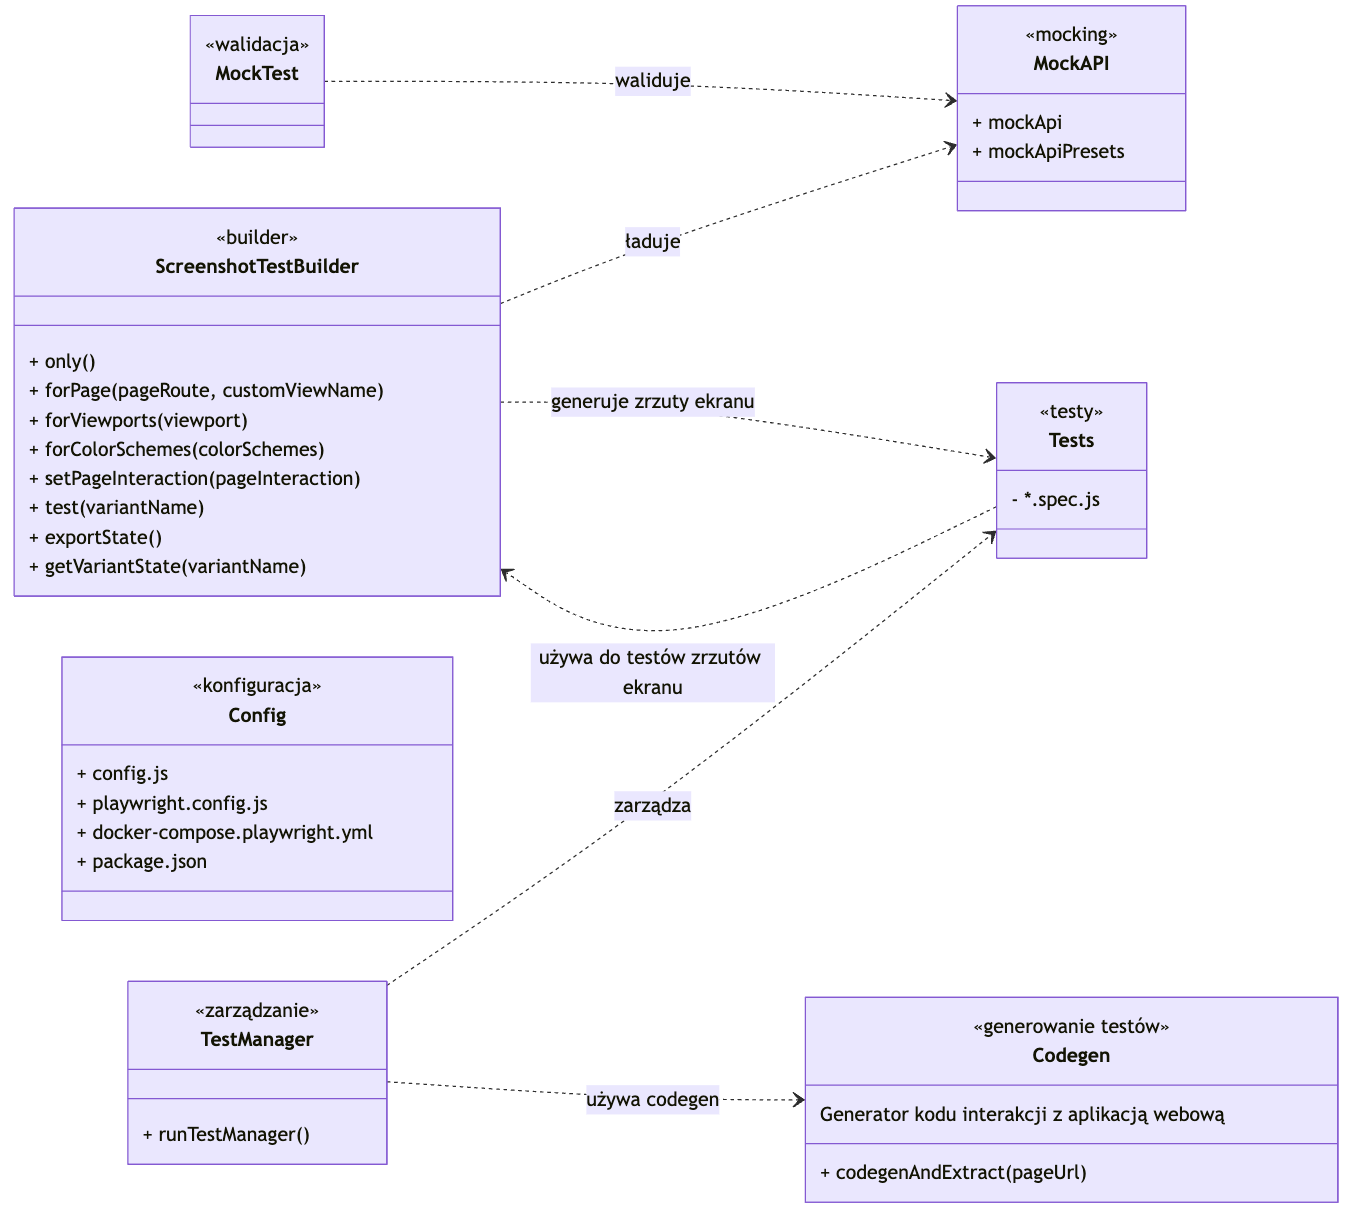
\includegraphics[width=0.95\textwidth]{diagram-projekt.png}
\caption{Diagram klas przedstawiający główne komponenty systemu}
\label{fig:diag-klas}
\end{figure}

Najważniejsze elementy widoczne na powyższym diagramie to:
\begin{itemize}
   \item \textbf{\texttt{ScreenshotTestBuilder}} -- centralny komponent służący do definiowania parametrów testów wizualnych (np.~rodzaje widoków, warianty kolorów, interakcje na stronie). Udostępnia metody umożliwiające budowanie kompletnego scenariusza testowego.
   \item \textbf{\texttt{Tests}} (zawartość plików \texttt{*.spec.js}) -- zestaw testów wykorzystujących przygotowane warianty i funkcje \texttt{ScreenshotTestBuilder}. Każdy test może generować zrzuty ekranu w różnych konfiguracjach (urządzenie \emph{desktop}/\emph{mobile}, tryb \emph{light}/\emph{dark}, konkretna przeglądarka itp.).
   \item \textbf{\texttt{TestManager}} -- narzędzie CLI do uruchamiania testów, zarządzania nimi (np.~edycja wariantów, usuwanie lub dodawanie interakcji) oraz współpracy z \texttt{codegen}.
   \item \textbf{\texttt{Codegen}} -- moduł pozwalający w półautomatyczny sposób wygenerować sekwencje interakcji z aplikacją (np.~kliknięcia i wypełnianie formularzy), które następnie mogą być użyte w testach \texttt{spec.js}.
   \item \textbf{\texttt{Config}} -- pliki konfiguracyjne projektu (np.~ustawienia rozdzielczości, ścieżki URL), dzięki którym w prosty sposób można dostosować testy do różnych środowisk.
   \item \textbf{\texttt{MockAPI}} i \textbf{\texttt{MockTest}} -- mechanizmy związane z symulowaniem wywołań API oraz walidacją, czy zdefiniowane dane \texttt{mock} są zgodne ze strukturą faktycznych odpowiedzi serwera.
\end{itemize}

\begin{figure}[H]
\centering
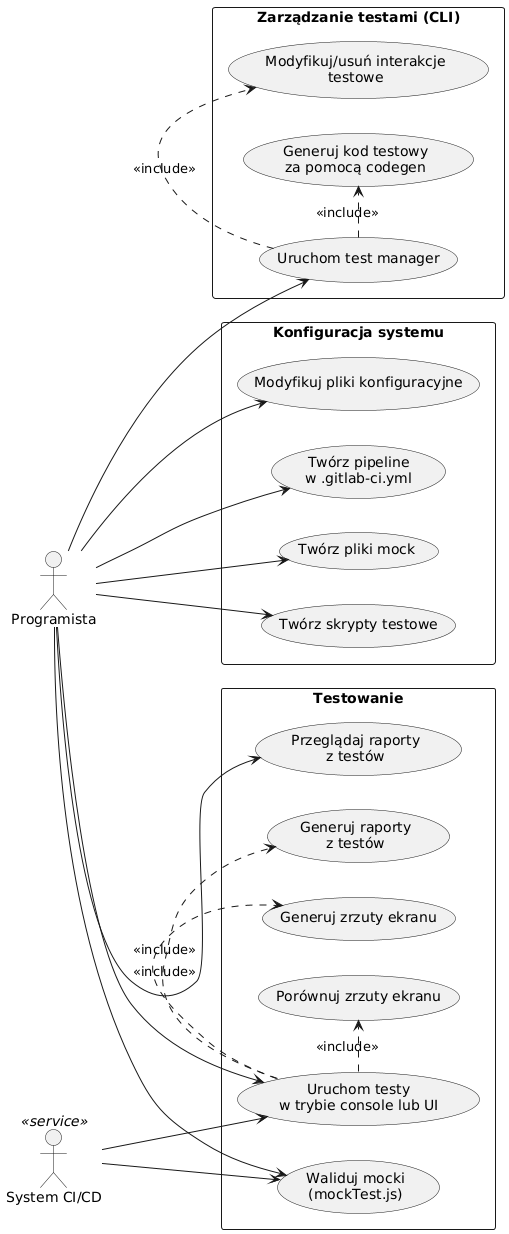
\includegraphics[width=0.7\textwidth]{use-uml.png}
\caption{Diagram przypadków użycia z perspektywy użytkownika i systemu CI/CD}
\label{fig:diag-use-case}
\end{figure}

Na diagramie przypadków użycia (rys.~\ref{fig:diag-use-case}) widoczna jest pełna interakcja pomiędzy:
\begin{itemize}
   \item \textbf{Programistą} -- tworzy i modyfikuje pliki konfiguracyjne, definiuje testy (\texttt{spec.js}) oraz może uruchamiać menedżer testów (\texttt{TestManager}).
   \item \textbf{Systemem CI/CD} -- automatycznie uruchamia testy (m.in.~testy zrzutów ekranu i walidacje \texttt{mock}), generuje raporty i zarządza pipeline’em.
\end{itemize}
Zarówno człowiek (Programista), jak i \emph{System CI/CD} korzystają z tych samych głównych operacji: uruchamianie testów, weryfikacja \texttt{mock} i przeglądanie raportów. Ponadto Programista może w dowolnym momencie wywołać \texttt{TestManager}, by zmodyfikować scenariusze testowe (np.~dodać nową interakcję na stronie).

\subsection{Zależność plików \texttt{spec.js} i \texttt{screenshotTestBuilder}}
\label{sec:zaleznosc-spec-builder}

Wszystkie pliki testowe oznaczone rozszerzeniem \texttt{.spec.js} w tym projekcie opierają się na funkcjonalnościach dostarczanych przez klasę \texttt{ScreenshotTestBuilder}. Oznacza to, że każdy test:
\begin{enumerate}
   \item Inicjalizuje \texttt{ScreenshotTestBuilder} (np.~wywołując konstruktor i metody konfiguracyjne \texttt{forPage}, \texttt{setPageInteraction} itp.),
   \item Definiuje warianty testów (\texttt{test()} z nazwą wariantu bądź bez),
   \item Przechowuje i wykorzystuje stan zdefiniowany przez \texttt{ScreenshotTestBuilder}, aby ostatecznie wygenerować zrzuty ekranu w różnych kombinacjach ustawień.
\end{enumerate}

\noindent \textbf{Ścisła zależność} między \texttt{spec.js} a \texttt{screenshotTestBuilder} polega na tym, że:
\begin{itemize}
   \item \texttt{screenshotTestBuilder} udostępnia metody pozwalające na łatwe ustawienie dowolnych parametrów testu (np.~\emph{viewport}, tryb kolorów, interakcje użytkownika),
   \item \texttt{*.spec.js} korzystają z tych metod w celu „zbudowania” gotowego scenariusza testowego,
   \item Każdy nowy plik \texttt{.spec.js} w praktyce \emph{musi} używać \texttt{ScreenshotTestBuilder}, dzięki czemu konfiguracja testów pozostaje spójna w całym projekcie.
\end{itemize}

\subsection{Rola \texttt{testManager} w zarządzaniu \texttt{spec.js} i codegenem}
\label{sec:rola-testManager}

\textbf{\texttt{testManager}} pełni w projekcie funkcję nadrzędnego narzędzia do zarządzania plikami \texttt{.spec.js} oraz wspiera Programistę w tworzeniu i modyfikowaniu interakcji testowych. Po uruchomieniu w trybie wiersza poleceń (CLI) pozwala m.in.:
\begin{itemize}
   \item \textbf{Przeglądać istniejące testy} -- użytkownik dostaje listę dostępnych plików \texttt{.spec.js} i może wybrać konkretny wariant testu do edycji.
   \item \textbf{Dodawać lub usuwać interakcje na stronie} -- \texttt{testManager} umożliwia szybkie wstawienie nowych kroków (np.~kliknięcie przycisku, wypełnienie formularza) lub wyeliminowanie dotychczasowych akcji.
   \item \textbf{Korzystać z \emph{codegen}} -- integracja z \emph{Playwright codegen} umożliwia półautomatyczne generowanie scenariuszy testowych. Codegen nie jest częścią autorską tego projektu, lecz stanowi wbudowane narzędzie \emph{Playwright} do rejestrowania czynności w przeglądarce. Dzięki \texttt{testManager}, Programista może wywołać codegen, który „nagrywa” kroki wykonywane na stronie, po czym wygenerowany kod może zostać łatwo włączony do pliku \texttt{.spec.js}.
\end{itemize}

Głównym zadaniem \texttt{testManager} jest więc ułatwienie nawigacji w wielu plikach testowych i wsparcie w zarządzaniu różnymi wariantami testów (np.~różne interakcje na tej samej stronie). Rozwiązuje to problem ręcznego dopisywania fragmentów kodu w \texttt{.spec.js}, bo dzięki integracji z codegen i mechanizmami CLI większość operacji można wykonać przy pomocy interaktywnych pytań i odpowiedzi.

\subsection{Działanie \texttt{mockApi} oraz \texttt{mockTest}}
\label{sec:dzialanie-mocki}

\textbf{\texttt{mockApi}} zapewnia w projekcie mechanizm definiowania sztucznych (testowych) odpowiedzi serwera. Dla wybranych endpointów API można zdefiniować, jakie dane mają być zwracane, dzięki czemu testy nie muszą opierać się na żywym środowisku produkcyjnym czy deweloperskim. Każda paczka \texttt{mock} (np.~\texttt{/home/home.mock.js}) zawiera:
\begin{itemize}
   \item \textbf{Dane do zwrócenia} -- statyczne lub wygenerowane, opisujące np.~przykładowy obiekt JSON, treść HTML czy obraz,
   \item \textbf{Parametry endpointu} -- wskazanie żądanej ścieżki (np.~\texttt{/branding/}) lub zapytania (\texttt{?query=test}),
   \item \textbf{Presety} -- grupowanie kilku \texttt{mock} w zestawy, które można jednocześnie załadować w testach (np.~\texttt{mockApiPresets.default}).
\end{itemize}

\noindent \textbf{\texttt{mockTest}} to z kolei moduł sprawdzający, czy zdefiniowane \texttt{mocki} są zgodne z prawdziwymi danymi, jakie zwraca produkcyjne API. Jego zadaniem jest:
\begin{itemize}
   \item \textbf{Pobranie realnej odpowiedzi} z wybranego endpointu w środowisku docelowym,
   \item \textbf{Porównanie struktury} z danymi zadeklarowanymi w \texttt{mockApi} (sprawdzana jest m.in.~zgodność typu pól czy format obrazów),
   \item \textbf{Raportowanie ewentualnych różnic} -- w razie niezgodności \texttt{mockTest} wskazuje, który \texttt{mock} wymaga aktualizacji, by odzwierciedlać rzeczywisty stan API.
\end{itemize}


\section{Szczegóły wybranych elementów (Rozdział 5.2)}
\label{sec:szczegoly-wybranych-elementow}

\subsection{API \texttt{screenshotTestBuilder} (metody \texttt{set}, \texttt{for} i inne) + przykład spec.js}
\label{sec:api-screenshotTestBuilder}
W tej części opisano najważniejsze metody dostępne w klasie \texttt{ScreenshotTestBuilder}. Dzięki nim można w przejrzysty sposób zdefiniować konfigurację testów wizualnych:

\begin{itemize}
  \item \texttt{only()} -- pozwala oznaczyć dany zestaw testów jako wykonywany \emph{wyłącznie} (z pominięciem innych).  
  \item \texttt{forPage(pageRoute, customViewName?)} -- określa, jaką trasę (URL) ma odwiedzić test i ew.~jaką nazwę widoku nadać danej konfiguracji (np.~\texttt{"home"}).
  \item \texttt{forViewports(viewport[])} -- ustawia listę viewportów (np.~\texttt{["desktop","mobile"]}).
  \item \texttt{forColorSchemes(colorSchemes[])} -- ustawia listę trybów kolorystycznych (np.~\texttt{["light","dark"]}).
  \item \texttt{setPageInteraction(async (page) => \{\ldots\})} -- umożliwia zdefiniowanie akcji wykonywanych na stronie przed zrobieniem zrzutu ekranu (np.~kliknięcie przycisku).
  \item \texttt{test(variantName?)} -- finalizuje konfigurację i tworzy właściwe testy (w kontekście \texttt{Playwright}). Parametr \texttt{variantName} służy do rozróżnienia różnych wariantów testu (np.~\texttt{"booking"}).
  \item \texttt{exportState()} -- zwraca obiekt z aktualnymi ustawieniami (np.~\texttt{pageRoute}, \texttt{viewport}, \texttt{colorSchemes}, \texttt{pageInteraction} itp.). Mechanizm wykorzystywany np.~przez \texttt{testManager}.
  \item \texttt{getVariantState(variantName)} -- zwraca zapisany stan konfiguracji dla wybranego \texttt{variantName}.
\end{itemize}

\noindent Przykładowy plik \texttt{example.spec.js}:

\begin{verbatim}
//@ts-check
import ScreenshotTest from '../screenshotTestBuilder.js';

new ScreenshotTest()
  .forPage('/', 'home')          // Ustawia główny adres / i nazywa ten widok "home"
  .forViewports(['desktop','mobile'])
  .forColorSchemes(['light','dark'])
  .setPageInteraction(async (page) => {
    await page.click('text=Akceptuj Cookies');
  })
  .test('accept-cookies')       // Pierwszy wariant testu (nazwa "accept-cookies")

  // Drugi wariant testu, inna interakcja
  .setPageInteraction(async (page) => {
    await page.click('text=Otwórz Menu');
  })
  .test('open-menu');
\end{verbatim}

W powyższym przykładzie zdefiniowano dwa warianty testu (\texttt{accept-cookies} oraz \texttt{open-menu}). Każdy z nich zostanie uruchomiony w dwóch trybach widoku (\emph{desktop}, \emph{mobile}) oraz dla dwóch schematów kolorów (\emph{light}, \emph{dark}). Łącznie wygeneruje to kilka zrzutów ekranu.

\subsection{Struktura plików \texttt{mock.js} (pola, za co odpowiadają) + przykład}
\label{sec:struktura-mockjs}
Pliki \texttt{.mock.js} odpowiadają za definiowanie odpowiedzi \emph{mockowanych} endpointów API. Każdy taki plik eksportuje zazwyczaj dwa obiekty:
\begin{itemize}
  \item \texttt{mockApi} -- zawiera definicje poszczególnych endpointów (np.~\texttt{branding}, \texttt{room}, \texttt{images}).
  \item \texttt{mockApiPresets} -- grupuje definicje w postaci zestawów, np.~\texttt{default}, \texttt{booking}, \texttt{error}.
\end{itemize}

\noindent Kluczowe pola w każdej definicji endpointu to:
\begin{itemize}
  \item \texttt{endpoint} -- ścieżka w API, np.~\texttt{'room/'}.
  \item \texttt{query} -- dodatkowe parametry zapytania (\texttt{'?page=1'}).  
  \item \texttt{data} -- treść, jaka zostanie zwrócona (obiekt JSON, tekst HTML, bufor obrazu).
  \item \texttt{contentType} -- typ \emph{Content-Type} odpowiedzi (\texttt{'application/json'}, \texttt{'image/jpeg'}, \texttt{'text/html'}).
  \item \texttt{apiUrl} (opcjonalne) -- jeśli \texttt{mock} ma wskazywać na inny adres bazowy niż domyślny.
\end{itemize}

\noindent Przykładowy plik \texttt{simple.mock.js}:

\begin{verbatim}
export const mockApi = {
  branding: {
    default: {
      endpoint: 'branding/',
      query: '',
      data: {
        name: 'Hotel Testowy',
        description: 'Najlepszy hotel w okolicy',
      },
      contentType: 'application/json'
    }
  },
  images: {
    logo: {
      endpoint: 'images/logo.png',
      query: '',
      data: Buffer.from([0x89, 0x50, 0x4e, 0x47]), // przykładowy bajt
      contentType: 'image/png'
    }
  }
};

export const mockApiPresets = {
  default: [
    mockApi.branding.default,
    mockApi.images.logo
  ]
};
\end{verbatim}

Dzięki \texttt{mockApiPresets.default} w testach można wczytać oba endpointy jednocześnie, co pozwala symulować środowisko bez konieczności korzystania z prawdziwej infrastruktury.


\subsection{Skrypty w \texttt{package.json}} % -- 5.2.3 ZMIENIONE
\label{sec:skrypty-package}

W pliku \texttt{package.json} zdefiniowano skrypty, które ułatwiają uruchamianie testów oraz zarządzanie projektem. Poniżej przedstawiono zawartość sekcji \texttt{"scripts"} wraz z krótkim omówieniem:

\begin{verbatim}
{
  "scripts": {
    "test:e2e": "playwright test",
    "test:e2e:docker": "docker-compose -f docker-compose.playwright.yml run --rm console",
    "test:e2e:ui": "playwright test --ui",
    "test:e2e:ui:docker": "docker-compose -f docker-compose.playwright.yml run --rm ui-mode",
    "manager": "node testManager.js",
    "test:mock": "node mockTest.js"
  }
}
\end{verbatim}

\begin{itemize}
    \item \texttt{"test:e2e"} -- uruchamia testy end-to-end za pomocą Playwright w trybie konsolowym.  
    \item \texttt{"test:e2e:docker"} -- podobne uruchomienie testów E2E, lecz w kontenerze (zdefiniowanym w \texttt{docker-compose.playwright.yml}) i z poleceniem \texttt{console}.
    \item \texttt{"test:e2e:ui"} -- wywołuje testy Playwright w trybie interfejsu graficznego (\texttt{--ui}), umożliwiając przeglądanie wyników testów w czasie rzeczywistym.
    \item \texttt{"test:e2e:ui:docker"} -- analogicznie jak wyżej, ale uruchamia się w środowisku Docker.
    \item \texttt{"manager"} -- wywołuje główne narzędzie CLI, czyli \texttt{testManager.js}, służące do interaktywnego zarządzania plikami \texttt{.spec.js} i wariantami testów.
    \item \texttt{"test:mock"} -- uruchamia \texttt{mockTest.js}, który weryfikuje poprawność \texttt{mockApi} w porównaniu do realnego API.
\end{itemize}

Dzięki tym skryptom można sprawnie kontrolować różne typy testów (E2E w kontenerze czy lokalnie, testy mocków) oraz korzystać z \texttt{testManager} bez konieczności ręcznego wpisywania dłuższych poleceń.


\subsection{\texttt{testManager}} % -- 5.2.4 ZMIENIONE
\label{sec:testManager}

Moduł \texttt{testManager} pełni rolę interfejsu CLI do zarządzania plikami testowymi (\texttt{.spec.js}) i ich wariantami. Pozwala m.in.:
\begin{itemize}
    \item Wybierać plik \texttt{.spec.js} z dostępnej listy,
    \item Odczytywać i modyfikować warianty testów w danym pliku,
    \item Dodawać lub usuwać interakcje użytkownika (\texttt{pageInteraction}),
    \item Uruchamiać \emph{Playwright codegen} w celu półautomatycznego wygenerowania nowych interakcji.
\end{itemize}

Poniżej pokazano przykładowe ekrany z działania \texttt{testManager}:

\begin{figure}[H]
\centering
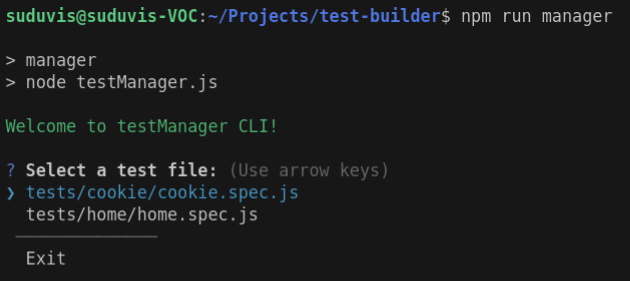
\includegraphics[width=0.93\textwidth]{tm_main_menu.png}
\caption{Główne menu \texttt{testManager} po uruchomieniu: użytkownik wybiera plik \texttt{.spec.js} lub opcję \textit{Exit}.}
\label{fig:tm_main_menu}
\end{figure}

Po wybraniu konkretnego pliku \texttt{.spec.js}, \texttt{testManager} wyświetla dostępne warianty testów:

\begin{figure}[H]
\centering
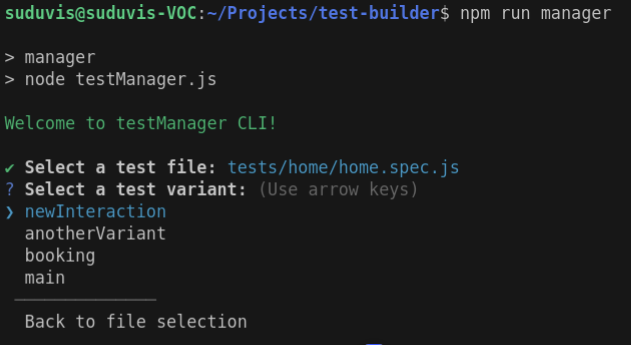
\includegraphics[width=0.93\textwidth]{tm_variant_selection_menu.png}
\caption{Menu wyboru wariantu w \texttt{testManager}. Można też wrócić do wyboru pliku \texttt{.spec.js}.}
\label{fig:tm_variant_selection_menu}
\end{figure}

Dla wybranego wariantu \texttt{testManager} prezentuje bieżącą konfigurację (widok, interakcje, wymiary itp.) w formie tabeli:

\begin{figure}[H]
\centering
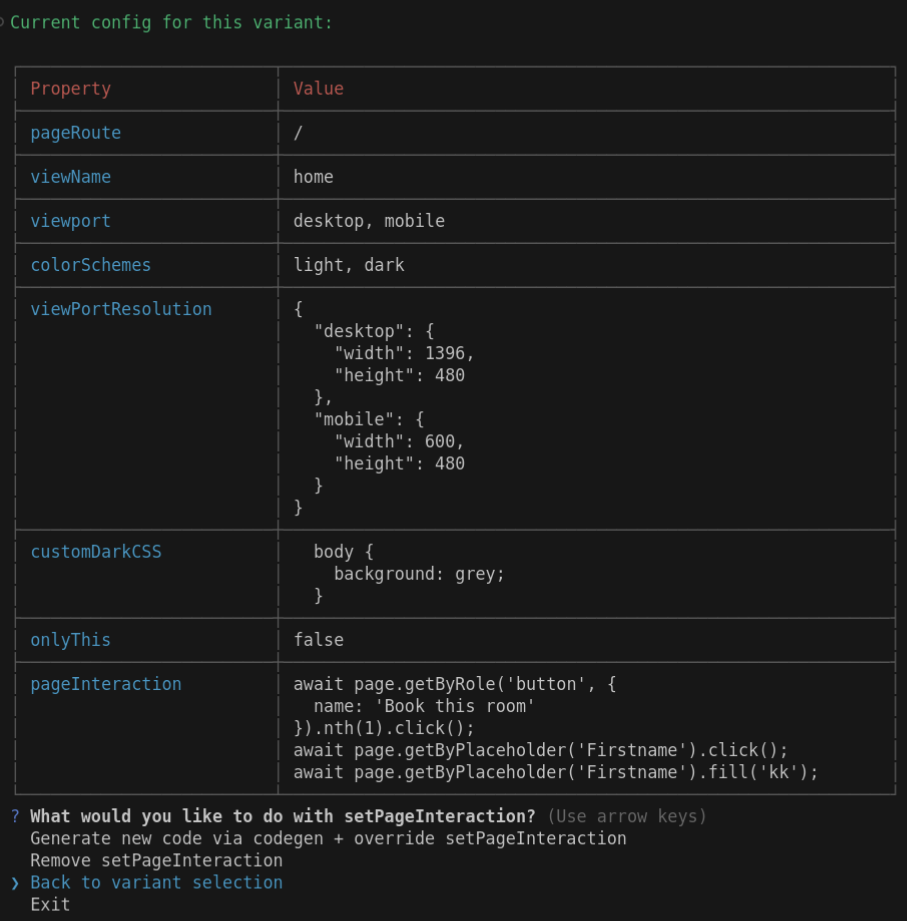
\includegraphics[width=0.93\textwidth]{tm_variant_details_menu.png}
\caption{Przykładowa tabelaryczna prezentacja stanu wariantu w \texttt{testManager}.}
\label{fig:tm_variant_details_menu}
\end{figure}

Następnie użytkownik może skorzystać z opcji:
\begin{itemize}
   \item \textbf{Generate new code via codegen + override \texttt{setPageInteraction}}:  
   wywołuje wewnętrznie \emph{Playwright codegen}, który otwiera przeglądarkę i rejestruje nowe czynności wykonywane przez testera. Po zakończeniu nagrywania \texttt{testManager} wstawia wygenerowany kod do \texttt{.spec.js}, zastępując dotychczasowy.
   \item \textbf{Remove \texttt{setPageInteraction}}:  
   usuwa z pliku \texttt{.spec.js} definicję akcji użytkownika dla bieżącego wariantu.
   \item \textbf{Back to variant selection / Exit}:  
   pozwala wrócić do poprzedniego kroku lub wyjść z narzędzia.
\end{itemize}

Rys.~\ref{fig:tm_code_generation} ilustruje moment, w którym \texttt{testManager} uruchamia przeglądarkę i \emph{Playwright codegen}, a użytkownik może „nagrać” nową sekwencję interakcji.

\begin{figure}[H]
\centering
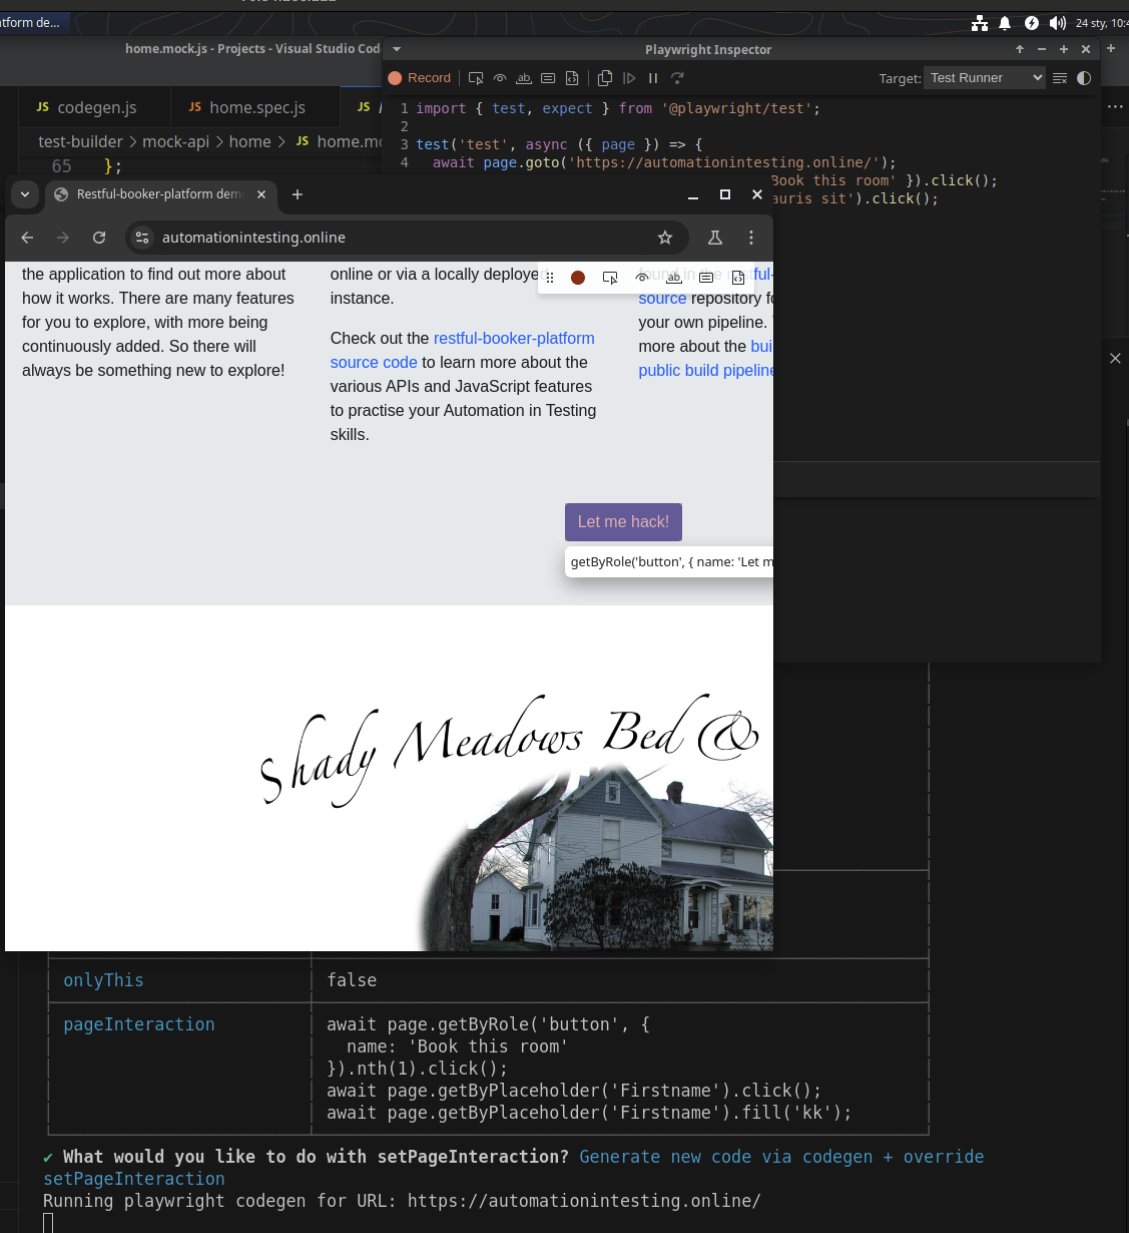
\includegraphics[width=0.95\textwidth]{tm_code_generation.png}
\caption{Przykład równoczesnego działania CLI \texttt{testManager} i \emph{Playwright codegen} (przeglądarka).}
\label{fig:tm_code_generation}
\end{figure}

\noindent Podsumowując, \texttt{testManager} upraszcza proces edycji i tworzenia testów:
\begin{enumerate}
   \item Interaktywnie prowadzi użytkownika przez wybór plików \texttt{.spec.js} i wariantów,
   \item Umożliwia szybkie przełączanie się między wariantami testów (bez konieczności ręcznego grzebania w kodzie),
   \item Zapewnia integrację z \emph{Playwright codegen}, dzięki czemu można łatwo „nagrać” nowe czynności na stronie i dołączyć je do testu,
   \item Pozwala na podgląd aktualnej konfiguracji (rozmiary ekranu, tryby kolorystyczne, akcje \texttt{pageInteraction} itp.) w czytelnej tabeli.
\end{enumerate}

Dzięki temu programiści oraz testerzy mogą w prosty sposób zarządzać dużą liczbą testów wizualnych (screen testów) i błyskawicznie wprowadzać zmiany w interakcjach wykonywanych przez test.


\chapter{Kluczowe mechanizmy i biblioteki}
\label{chap:kluczowe-mechanizmy}

W niniejszym rozdziale omówione zostaną kluczowe elementy rozwiązania wspierającego automatyzację testów aplikacji webowych. Przedstawiono tutaj sposób organizacji zasobów projektowych (folderów i plików), zasady definiowania nazw zrzutów ekranu oraz kluczowe mechanizmy umożliwiające generowanie i wykonywanie testów \texttt{E2E} w oparciu o narzędzie \texttt{Playwright}. Opisano też rolę menedżera testów (\texttt{testManager}) wraz z integracją mechanizmu \texttt{codegen}, a także koncepcję weryfikacji plików \texttt{mock} względem faktycznych odpowiedzi serwera (\texttt{mockTest}). Na zakończenie rozdziału podkreślono, jakich bibliotek użyto do implementacji poszczególnych modułów oraz wskazano najważniejsze miejsca w kodzie, w których zaimplementowano prezentowane mechanizmy.

\section{Zasady organizacji projektu}
\label{sec:zasady-organizacji}

\subsection{Struktura folderów i plików projektu; nazewnictwo zrzutów ekranu}
\label{sec:struktura-folderow}

W projekcie wyróżnić można kilka istotnych katalogów, zorganizowanych w taki sposób, aby ułatwić utrzymanie testów, mocków oraz plików konfiguracyjnych:

\begin{itemize}
    \item \textbf{\texttt{/tests}} -- tutaj znajdują się właściwe testy \texttt{.spec.js} wraz z wygenerowanymi zrzutami ekranu. Każdy scenariusz testowy może zostać osadzony w dedykowanym podfolderze (np.~\texttt{/tests/home}, \texttt{/tests/cookie}), co pozwala na tematyczne grupowanie testów.
    \begin{itemize}
        \item Każdy \texttt{.spec.js} test może generować wiele zrzutów ekranu. Zrzuty te, zgodnie z konfiguracją, przechowywane są w tym samym folderze, co plik testowy (np.~\texttt{home.spec.js} obok plików \texttt{home-desktop-light-chromium.png}).
    \end{itemize}
    \item \textbf{\texttt{/mock}} (\texttt{mock-api}) -- w tym katalogu znajdują się pliki \texttt{.mock.js} opisujące zachowania poszczególnych endpointów (np.~\texttt{home.mock.js}, \texttt{cookie.mock.js}). Dzięki nim testy mogą działać bez konieczności nawiązywania połączenia z realnym środowiskiem serwerowym.
    \item \textbf{\texttt{config.js}, \texttt{playwright.config.js}, \texttt{docker-compose.playwright.yml}} -- pliki odpowiedzialne za konfigurację środowiska, ustawienia \texttt{Playwright} oraz ewentualną orkiestrację w kontenerach Docker.
    \item \textbf{\texttt{testManager.js}, \texttt{screenshotTestBuilder.js}, \texttt{mockTest.js}} -- najistotniejsze skrypty odpowiedzialne za mechanizmy opisywane w niniejszym rozdziale, tj.~zarządzanie testami, generowanie zrzutów ekranu i weryfikację \texttt{mock}.
\end{itemize}

\noindent \textbf{Sposób nazywania zrzutów ekranu.}  
Wygenerowane zrzuty ekranu w katalogu \texttt{/tests} posiadają nazwy zgodne ze schematem:
\[
    \texttt{viewName-viewport-colorscheme-variant-przegladarka.png}
\]
gdzie:
\begin{itemize}
    \item \texttt{viewName} -- nazwa widoku bądź strony, np.~\texttt{home} lub \texttt{cookie};
    \item \texttt{viewport} -- informacja o rodzaju wyświetlacza, np.~\texttt{desktop} bądź \texttt{mobile};
    \item \texttt{colorscheme} -- \texttt{light} lub \texttt{dark}, zależnie od tematu kolorystycznego;
    \item \texttt{variant} -- opcjonalna etykieta, np.~\texttt{booking} oznaczająca konkretny scenariusz w obrębie tej samej strony;
    \item \texttt{przegladarka} -- wskazanie, w jakiej przeglądarce dany zrzut został wykonany (np.~\texttt{chromium}, \texttt{firefox}, \texttt{webkit}).
\end{itemize}

Przykładowo nazwa \texttt{home-desktop-light-booking-chromium.png} oznacza, że jest to zrzut strony \texttt{home}, wykonany w trybie \texttt{desktop}, przy jasnej kolorystyce (\texttt{light}) i wariancie testu \texttt{booking}, w przeglądarce \texttt{chromium}. Taki sposób nazywania ułatwia szybkie odnalezienie odpowiedniej kombinacji parametrów wśród wielu plików screenshotów.

\subsection{Mechanizm tworzenia testów E2E przez \texttt{screenshotTestBuilder}}
\label{sec:mechanizm-builder}

Proces tworzenia testów E2E z wykorzystaniem \texttt{Playwright} jest w projekcie wspierany przez komponent \texttt{screenshotTestBuilder}. Pomysł polega na tym, aby w jednym miejscu deklarować \emph{parametry} testu (np.~jaką stronę należy odwiedzić, w jakich wymiarach przeglądarki, z jakim schematem kolorów, jakie interakcje powinny zostać wykonane), a następnie na tej podstawie automatycznie zbudować gotowy skrypt \texttt{.spec.js}.

W praktyce wygląda to następująco:
\begin{enumerate}
    \item \textbf{Inicjacja buildera:} w pliku \texttt{.spec.js} tworzy się nowy obiekt \texttt{ScreenshotTest()}, co stanowi punkt wyjścia do konfiguracji testu.
    \item \textbf{Ustawianie parametrów:} za pomocą metod takich jak \texttt{forPage()}, \texttt{forViewports()}, \texttt{forColorSchemes()} programista wskazuje, jakie warianty (viewporty, tryby kolorystyczne) mają zostać uwzględnione.
    \item \textbf{Opcjonalne interakcje:} \texttt{setPageInteraction()} pozwala zdefiniować akcje wykonywane na stronie (np.~kliknięcia, wypełnianie formularza) przed zrobieniem zrzutu ekranu.
    \item \textbf{Deklaracja testu:} wywołanie \texttt{test()} zamyka konfigurację i generuje serię rzeczywistych testów \texttt{Playwright} (po jednym na każdą kombinację viewportu, trybu kolorystycznego, nazwy wariantu itd.).
    \item \textbf{Uruchomienie:} w trakcie wykonywania testów (\texttt{npx playwright test}) aplikacja odwiedza wskazaną stronę, wywołuje zadane interakcje i zapisuje zrzuty ekranu w odpowiednich plikach (zgodnie z opisanym wcześniej schematem nazewnictwa).
\end{enumerate}

Dzięki temu mechanizmowi programista nie musi tworzyć wielu osobnych plików testowych dla każdej kombinacji rozdzielczości, koloru czy wariantu scenariusza. Zamiast tego jeden builder potrafi wygenerować i uruchomić szereg analogicznych testów o wspólnych parametrach. Dodatkowo, \texttt{ScreenshotTestBuilder} pozwala na \emph{eksport} konfiguracji (np.~by wykorzystać ją w \texttt{testManager}), co znacznie ułatwia edycję i utrzymanie testów w dłuższym okresie.

\subsection{Mechanizm \texttt{testManager} z wykorzystaniem \texttt{codegen}}
\label{sec:mechanizm-testManager}

\textbf{Mechanizm, w którym \texttt{testManager} wykorzystuje \texttt{codegen} do tworzenia skryptu z interakcją na stronie, bazujący na obiekcie \texttt{page}, przebiega następująco:}

\begin{enumerate}
    \item \textbf{Wybór pliku i wariantu testu w CLI:} Użytkownik uruchamia \texttt{testManager} w trybie wiersza poleceń. Narzędzie skanuje katalog \texttt{/tests}, odnajduje wszystkie pliki \texttt{.spec.js} i wyświetla ich listę. Po wybraniu konkretnego pliku, \texttt{testManager} pokazuje dostępne warianty testu (zdefiniowane metodą \texttt{test('nazwaWariantu')} w kodzie \texttt{.spec.js}).
    \item \textbf{Wywołanie opcji generowania interakcji:} Gdy użytkownik chce zmodyfikować lub dodać nową sekwencję interakcji w danym wariancie, wybiera w menu opcję „Generate new code via codegen + override \texttt{setPageInteraction}”. 
    \item \textbf{Uruchomienie \emph{Playwright codegen}:} \texttt{testManager} w tle wykonuje polecenie \texttt{npx playwright codegen <URL>}, gdzie \texttt{<URL>} to z reguły \texttt{basePageUrl + pageRoute} (ustalone w konfiguracji testu). Otwiera się przeglądarka w trybie interaktywnym oraz dodatkowe okno z wygenerowanym kodem.
    \item \textbf{Rejestrowanie akcji użytkownika:} Wszystkie kliknięcia, wypełnienia pól formularza, nawigacja itp. są w czasie rzeczywistym zapisywane w kodzie JavaScript/TypeScript (zależnie od ustawień). \emph{Playwright codegen} generuje m.in. sekwencje wywołań \texttt{page.click()}, \texttt{page.fill()} i tym podobnych.
    \item \textbf{Zapisanie wygenerowanego kodu:} Po zakończeniu „nagrywania” interakcji, \texttt{codegen} tworzy tymczasowy plik, z którego \texttt{testManager} odczytuje potrzebne fragmenty (zwykle samą zawartość funkcji asynchronicznej wykorzystującej obiekt \texttt{page}).
    \item \textbf{Nadpisanie \texttt{setPageInteraction} w pliku \texttt{.spec.js}:} \texttt{testManager} analizuje obecny kod \texttt{.spec.js}, odnajduje właściwy blok \texttt{setPageInteraction(async (page) => \{...\})} dla wybranego wariantu testu i wstawia tam nowo wygenerowaną treść (czyli ciąg wywołań \texttt{page.XXX()}). 
    \item \textbf{Formatowanie i zapis zmian:} Na końcu \texttt{testManager} może wywołać \texttt{prettier} (jeśli jest dostępny), aby kod testu zachował spójny styl. Zmodyfikowany plik \texttt{.spec.js} zostaje nadpisany, co oznacza, że kolejny \texttt{test:e2e} będzie wykonywał już zaktualizowane kroki.
    \item \textbf{Potwierdzenie w CLI:} Użytkownik widzi w \texttt{testManager} informację, że interakcja została zmieniona. Może teraz w dowolnym momencie uruchomić \texttt{npx playwright test} (albo skorzystać z pipeline’u CI) i sprawdzić działanie nowego scenariusza.
\end{enumerate}

\noindent Dzięki temu procesowi \texttt{testManager} \emph{integruje} się z wbudowanym w Playwright narzędziem \texttt{codegen}, pozwalając w szybki sposób tworzyć lub modyfikować \emph{krok po kroku} akcje \texttt{page}, które zostaną wykonane w testach. Jest to szczególnie przydatne dla osób, które nie chcą ręcznie pisać skryptów interakcji z przeglądarką, a wolą nagrać je przez klikanie w interfejs.

\subsection{Mechanizm działania \texttt{mockTest}}
\label{sec:mechanizm-mocktest}

\textbf{Moduł \texttt{mockTest}} sprawdza, czy pliki \texttt{.mock.js} (odpowiedzialne za symulowanie wywołań API) są zgodne ze strukturą i danymi zwracanymi przez realne API. Mechanizm jego działania można podzielić na następujące kroki:

\begin{enumerate}
    \item \textbf{Wczytanie wszystkich plików \texttt{.mock.js}:} \texttt{mockTest} rekurencyjnie przegląda katalog \texttt{mock-api} i importuje każdy plik definiujący \texttt{mockApi} oraz \texttt{mockApiPresets}. Dzięki temu uzyskuje listę wszystkich endpointów, które w testach mogą być symulowane.
    \item \textbf{Dla każdego endpointu - pobranie faktycznej odpowiedzi API:} \texttt{mockTest} odczytuje z \texttt{mockApi} m.in. \texttt{endpoint}, \texttt{query} oraz ewentualny \texttt{apiUrl}, a następnie wykonuje żądanie HTTP do prawdziwego serwera (zdefiniowanego np. w \texttt{config.js} jako \texttt{baseApiUrl}).  
    \item \textbf{Porównanie \emph{Content-Type} i danych:}  
    \begin{itemize}
        \item Jeśli \texttt{contentType} to obraz (\texttt{image/png}, \texttt{image/jpeg}), \texttt{mockTest} pobiera dane w postaci binarnej i porównuje bajt po bajcie z tym, co jest w \texttt{mockApi}.  
        \item Jeśli \texttt{contentType} to \texttt{application/json}, \texttt{mockTest} konwertuje odpowiedź na obiekt JSON i sprawdza, czy struktura (schemat) odpowiada danym określonym w \texttt{mockApi}. Wykorzystywane są do tego takie narzędzia jak \texttt{ajv} (JSON schema validator) czy \texttt{quicktype-core} (do generowania schematu na podstawie przykładowych danych).
    \end{itemize}
    \item \textbf{Walidacja różnic i raportowanie:} Jeśli \texttt{mockTest} wykryje, że \emph{struktura} JSON różni się od tej, którą deklaruje \texttt{mockApi} (np. brakuje jakiegoś pola w obiekcie, ma inny typ lub nazwa klucza się nie zgadza), wówczas generuje komunikat o błędzie. Analogicznie w przypadku obrazów – jeśli zawartość bajtów nie pasuje, test również uznawany jest za niepoprawny.
    \item \textbf{Informacja zwrotna na temat ewentualnych poprawek:} Programista po uruchomieniu \texttt{node mockTest.js} dostaje w konsoli informację, czy wszystkie \texttt{mocki} są zgodne z aktualnym stanem API, a jeśli nie – w których konkretnie polach czy plikach \texttt{mock.js} pojawiły się rozbieżności.
\end{enumerate}

\noindent Istotną zaletą \texttt{mockTest} jest to, że \emph{uniemożliwia} długotrwałe utrzymywanie nieaktualnych plików \texttt{mock.js}, co zapobiega sytuacji, w której testy przechodzą tylko dlatego, że używają zastarzałej, błędnej symulacji API. W momencie, gdy rzeczywiste API ulega zmianie (np. dodaje nowe pola w JSON), od razu wiadomo, że \texttt{mockTest} tego nie przepuści i wymusi dostosowanie \texttt{mockApi} do nowego formatu.

\section{Omówienie kluczowych bibliotek}
\label{sec:omowienie-bibliotek}

W projekcie wykorzystano szereg bibliotek oraz narzędzi, które wspomagają proces automatyzacji testów aplikacji webowych, zarówno od strony przygotowywania i uruchamiania scenariuszy E2E, jak i zarządzania nimi czy walidacji danych zwracanych przez API. Poniżej przedstawiono najważniejsze z nich wraz z opisem roli, jaką pełnią w systemie:

\begin{itemize}
    \item \textbf{Playwright} (\verb|@playwright/test|) -- podstawowa technologia do testów E2E w tym projekcie. Umożliwia uruchamianie testów w przeglądarkach Chromium, Firefox oraz WebKit. Dostarcza wbudowanego \emph{test runnera}, obsługę zrzutów ekranu, generowanie raportów (także w trybie interfejsu graficznego) oraz narzędzie \emph{codegen} do interaktywnego rejestrowania akcji użytkownika.

    \item \textbf{Inquirer} -- biblioteka do tworzenia interaktywnych menu w wierszu poleceń (CLI). Z jej pomocą zaimplementowano \texttt{testManager}, który pyta użytkownika o wybór plików \texttt{.spec.js}, wariantów testów oraz pozwala na zarządzanie interakcjami. 

    \item \textbf{Chalk} -- pakiet do kolorowania i formatowania tekstu w konsoli. Dzięki niemu \texttt{testManager} może wyświetlać wyróżnione komunikaty (np.~z powodzeniem, ostrzeżenia, błędy), zwiększając czytelność i wygodę obsługi narzędzia.

    \item \textbf{Prettier} -- narzędzie do automatycznego formatowania kodu JavaScript/TypeScript. Po nagraniu akcji w \emph{Playwright codegen}, \texttt{testManager} może wywołać \texttt{prettier} w celu znormalizowania stylu wygenerowanego kodu i wstawienia go w pliku \texttt{.spec.js}. Ułatwia to utrzymanie jednolitego stylu całego repozytorium.

    \item \textbf{Babel} (w szczególności \verb|@babel/parser|, \verb|@babel/traverse|, \verb|@babel/types| i \verb|@babel/generator|) -- zestaw narzędzi do parsowania kodu JavaScript i dokonywania w nim modyfikacji w postaci drzewa AST (\emph{Abstract Syntax Tree}). W \texttt{testManager} wykorzystuje się Babel do:
    \begin{enumerate}
        \item Odczytu istniejących plików \texttt{.spec.js} i odnajdywania miejsc, w których występują wywołania \texttt{test()} oraz \texttt{setPageInteraction(...)}.
        \item Nadpisywania fragmentów kodu, np.~wstawiania nowo wygenerowanej sekwencji akcji z \emph{codegen} (tj.~ciągu wywołań \verb|page.click(...)|, \verb|page.fill(...)| itp.).
        \item Generowania zaktualizowanego pliku testowego, który zostaje ostatecznie zapisany na dysku.
    \end{enumerate}

    \item \textbf{cli-table3} -- pakiet pozwalający wyświetlać w konsoli dane w formie tabelarycznej. W \texttt{testManager} używany do prezentacji aktualnej konfiguracji wybranego wariantu testu (np.~rozmiar viewportu, kolor, nazwa interakcji). Ułatwia to szybki wgląd w kluczowe parametry.

    \item \textbf{AJV} (\emph{Another JSON Validator}) oraz \textbf{ajv-formats} -- biblioteki do walidacji struktury danych w formacie JSON. Służą one \texttt{mockTest} do sprawdzania, czy dane zwracane przez \texttt{mockApi} pokrywają się ze schematem danych realnego API.

    \item \textbf{quicktype-core} -- narzędzie umożliwiające na podstawie przykładowego JSON-u (pobranego z produkcyjnego API) automatyczne wyprowadzenie schematu (\emph{JSON Schema}), który następnie jest weryfikowany z \texttt{mockApi}. \texttt{mockTest} korzysta z \emph{quicktype-core} do inferencji tego schematu w locie i porównywania go z danymi zadeklarowanymi w pliku \texttt{.mock.js}.

    \item \textbf{node-fetch} -- biblioteka do wykonywania zapytań HTTP po stronie Node.js. Wykorzystywana w \texttt{mockTest} przy pobieraniu realnych danych z API, aby sprawdzić aktualną strukturę i porównać ją z zawartością \texttt{mockApi}.

    \item \textbf{Docker / Docker-Compose} -- środowisko konteneryzacji (z plikiem \texttt{docker-compose.playwright.yml}), w którym można uruchomić testy E2E w odizolowanym kontenerze. Pozwala to zapewnić spójne i powtarzalne warunki uruchomieniowe (m.in.~zdefiniowana wersja \verb|mcr.microsoft.com/playwright|). 

\end{itemize}

Wszystkie wymienione wyżej biblioteki są zdefiniowane w pliku \texttt{package.json} (sekcja \texttt{dependencies}) i instalowane wraz z projektem (\verb|npm install|). Ich dobór podyktowany był dążeniem do zapewnienia:
\begin{itemize}
    \item \textbf{Spójnego ekosystemu testowego} -- \emph{Playwright} gwarantuje solidną podstawę do automatyzacji E2E, wspieraną przez narzędzia do walidacji i generowania scenariuszy.
    \item \textbf{Wysokiej czytelności i automatyzacji} -- \emph{Inquirer}, \emph{Chalk} i \emph{cli-table3} umożliwiają tworzenie rozbudowanego, przyjaznego CLI, a \emph{Babel} i \emph{Prettier} pozwalają na automatyczną modyfikację i formatowanie kodu.
    \item \textbf{Łatwej integracji z różnymi środowiskami} -- \emph{Docker-Compose} w połączeniu z obrazem \texttt{playwright} ułatwia uruchamianie testów na dowolnej maszynie, w tym w pipeline’ach CI/CD.
\end{itemize}

Zastosowanie powyższych bibliotek i narzędzi w sposób synergiczny pozwoliło na uzyskanie rozwiązania, w którym zarówno interaktywna konfiguracja, jak i sam proces testowania (od generowania kodu aż po sprawdzanie poprawności danych) działają płynnie i elastycznie.

\subsection{Kluczowe miejsca w kodzie}
\label{sec:6.3}

W poniższym podrozdziale zaprezentowano i omówiono cztery kluczowe fragmenty kodu źródłowego projektu, które w szczególny sposób ilustrują mechanizmy związane z tworzeniem testów, generowaniem interakcji i mockowaniem odpowiedzi API. Są to:

\begin{itemize}
  \item metoda \verb|#mockApiCall|,
  \item metoda \verb|test(variantName)|,
  \item funkcja \verb|inferSchemaFromJSON(jsonData)|,
  \item funkcja \verb|codegenAndExtract(pageUrl)|.
\end{itemize}

Każdy fragment został przytoczony w formie kodu oraz wzbogacony o komentarz wyjaśniający jego działanie i zastosowanie w projekcie.

\subsubsection{Metoda \texttt{\#mockApiCall}}
\label{sec:mockApiCall}

\begin{verbatim}
async #mockApiCall(page) {
  const mockApi = await getMockDataFor(this.#viewName);
  const { mockApiPresets } = mockApi;

  for (const {
    endpoint,
    data,
    contentType,
    customQuery = '',
    apiUrl,
  } of mockApiPresets.default) {
    await page.route(
      `${apiUrl || config.baseApiUrl}/${endpoint}${customQuery}`,
      async (route) => {
        if (contentType === 'text/html') {
          await route.fulfill({
            contentType: 'text/html',
            body: data,
          });
        } else if (contentType?.startsWith('image/')) {
          await route.fulfill({
            contentType: contentType,
            body: data,
          });
        } else {
          await route.fulfill({ json: data });
        }
      }
    );
  }
}
\end{verbatim}

\noindent
\textbf{Opis działania:}\\
Powyższa metoda \verb|#mockApiCall| (zaimplementowana w klasie \verb|ScreenshotTestBuilder|) umożliwia podstawienie zdefiniowanych wcześniej \textit{mocków} API zamiast prawdziwych wywołań sieciowych. Dzięki temu test nie musi odwoływać się do realnego serwera. Mechanizm w kolejnych krokach:

\begin{enumerate}
  \item Odczytuje dane z pliku \verb|.mock.js| przypisanego do aktualnie testowanego widoku (\verb|this.#viewName|).
  \item Iteruje po wszystkich wpisach w \verb|mockApiPresets.default|, które opisują m.in. \verb|endpoint|, \verb|contentType| i same \verb|data|.
  \item Dla każdej ścieżki \verb|endpoint| (oraz parametrów \verb|query|) rejestruje \texttt{page.route}, aby przechwycić żądanie do API w trakcie testu.
  \item Wywołuje \verb|route.fulfill(...)|, zwracając przygotowany \textit{mock}:
    \begin{itemize}
      \item tekst/HTML (\texttt{'text/html'}),
      \item obraz (\texttt{'image/...'}) lub
      \item obiekt JSON.
    \end{itemize}
\end{enumerate}

Dzięki temu możliwe jest wiarygodne testowanie \textit{front-endu} bez dostępu do prawdziwych zasobów sieciowych, a wyniki testów (np. zrzuty ekranu) nie są zależne od stanu środowiska zewnętrznego.

\subsubsection{Metoda \texttt{test(variantName)}}
\label{sec:test_variantName}

\begin{verbatim}
test(variantName) {
  if (!this.#pageRoute) throw new Error('Page route is not set');

  const isCli = process.env.SCREENSHOT_TEST_BUILDER_CLI === 'true';

  if (!isCli) {
    const testFunction = this.#onlyThis ? t.only : t;

    const testCases = variantName ? [variantName] : [null];
    const testState = {
      pageInteraction: this.#pageInteraction,
    };

    for (const viewPort of this.#viewport) {
      for (const colorScheme of this.#colorSchemes) {
        for (const variant of testCases) {
          testFunction(
            this.#getTestDescription(viewPort, colorScheme, variant),
            async ({ page }) => {
              await this.#mockApiCall(page);
              await this.#setViewportFor(viewPort, page);
              await this.#setColorScheme(colorScheme, page);
              await page.goto(this.#pageRoute);
              await testState.pageInteraction?.(page);

              await expect(page).toHaveScreenshot(
                this.#getReferenceFileFor(viewPort, colorScheme, variant),
                { fullPage: true }
              );
            }
          );
        }
      }
    }
  }

  const usedVariantName = variantName || 'main';
  this.#variantsState[usedVariantName] = this.exportState();

  this.#resetState();
  return this;
}
\end{verbatim}

\noindent
\textbf{Opis działania:}\\
Metoda \verb|test(variantName)| pełni kluczową rolę w generowaniu i wykonywaniu właściwych testów w oparciu o Playwright. Każdorazowe wywołanie:
\begin{itemize}
  \item Sprawdza, czy określono \verb|this.#pageRoute| (adres strony do odwiedzenia).
  \item Rozróżnia, czy test ma zostać uruchomiony normalnie, czy w trybie CLI (\texttt{isCli}).
  \item Dla zadanych kombinacji \verb|viewPort|, \verb|colorSchemes| oraz dla konkretnej nazwy wariantu (\verb|variantName| lub \verb|null|) tworzy wewnątrz pętlę:
    \begin{itemize}
      \item \verb|testFunction(...)| to tak naprawdę wywołanie \verb|test(...)| lub \verb|test.only(...)| z Playwright (\verb|t.only|).
      \item Wywołuje \verb|#mockApiCall|, by \textbf{podmienić} ewentualne wywołania sieciowe.
      \item Ustawia rozdzielczość (\verb|#setViewportFor|) oraz schemat kolorów (\verb|#setColorScheme|).
      \item Otwiera stronę \verb|this.#pageRoute| (\verb|page.goto(...)|) i wykonuje \textit{interakcję} (\verb|this.#pageInteraction|).
      \item Kończy się asercją \verb|expect(page).toHaveScreenshot(...)|, co generuje i porównuje zrzut ekranu.
    \end{itemize}
  \item Na zakończenie zapisuje stan konfiguracji (\verb|#variantsState|) i czyści \verb|#pageInteraction| (\verb|#resetState|).
\end{itemize}

W efekcie programista może wywołać \verb|.test(...)| dla różnych wariantów (np. \texttt{'booking'}), a każdy z nich spowoduje wykonanie jednej lub wielu kombinacji testowych (różne przeglądarki, rozdzielczości, kolory).

\subsubsection{Funkcja \texttt{inferSchemaFromJSON(jsonData)}}
\label{sec:inferSchemaFromJSON}

\begin{verbatim}
async function inferSchemaFromJSON(jsonData) {
  const jsonInput = jsonInputForTargetLanguage('schema');
  await jsonInput.addSource({
    name: 'GeneratedSchema',
    samples: [JSON.stringify(jsonData)],
  });

  const inputData = new InputData();
  inputData.addInput(jsonInput);

  const { lines } = await quicktype({
    inputData,
    lang: 'schema',
  });

  return lines.join('\n');
}
\end{verbatim}

\noindent
\textbf{Opis działania:}\\
Funkcja \verb|inferSchemaFromJSON| (obecna w \texttt{mockTest.js}) korzysta z biblioteki \emph{quicktype-core} w celu automatycznego wyprowadzenia schematu (JSON Schema) na podstawie przykładowych danych JSON. W skrócie:

\begin{enumerate}
  \item Tworzony jest obiekt \verb|jsonInputForTargetLanguage('schema')|, do którego \emph{dodaje się} przykładowe dane \verb|jsonData|.
  \item Następnie \verb|inputData| (klasa \verb|InputData| z \emph{quicktype}) zostaje wypełniona tym źródłem.
  \item Wywołanie \verb|quicktype(...)| generuje linie (tekst) zawierające schemat w formacie JSON Schema.
  \item Funkcja zwraca całość w formie spójnego łańcucha znaków (\texttt{lines.join('\n')}).
\end{enumerate}

Ten schemat jest dalej wykorzystywany do walidacji \emph{mocków} w \texttt{mockTest}, aby sprawdzić, czy struktura \texttt{mockApi} \textbf{odpowiada} realnemu formatowi z produkcyjnego API.

\subsubsection{Funkcja \texttt{codegenAndExtract(pageUrl)}}
\label{sec:codegenAndExtract}

\begin{verbatim}
export async function codegenAndExtract(pageUrl) {
  const inputFile = path.join(__dirname, 'input.js');

  try {
    console.log(`Running playwright codegen for URL: ${pageUrl}`);
    await executeCommand(
      `npx playwright codegen ${pageUrl} --output=${inputFile}`
    );
    console.log('Playwright codegen completed.');

    const extractedCode = await parseInputFile(inputFile);

    await fs.promises.unlink(inputFile);
    console.log(`Removed temporary file: ${inputFile}`);

    return extractedCode;
  } catch (err) {
    console.error('An error occurred during codegen:', err);
    throw err;
  }
}
\end{verbatim}

\noindent
\textbf{Opis działania:}\\
Funkcja \verb|codegenAndExtract| (z pliku \verb|codegen.js|) stanowi interfejs do wbudowanego w Playwright \texttt{codegen}, który nagrywa akcje wykonywane w przeglądarce:

\begin{enumerate}
  \item Uruchamia zewnętrzny proces \texttt{npx playwright codegen} dla podanego \verb|pageUrl|, wskazując \verb|--output| na tymczasowy plik \verb|input.js|.
  \item Po zakończeniu rejestracji \texttt{codegen} wytwarza kod (zwykle zestaw wywołań \verb|page.click(...)|, \verb|page.fill(...)| itp.).
  \item Następnie \verb|parseInputFile| (wewnętrzna funkcja) wyodrębnia istotne fragmenty ze wspomnianego \verb|input.js|.
  \item Plik tymczasowy jest usuwany, a funkcja zwraca gotowy kod \emph{(string)} – który może być wstawiony np. do \verb|setPageInteraction| przez \texttt{testManager}.
\end{enumerate}

Dzięki temu podejściu można \emph{nagrywać} kroki wykonywane na stronie, a następnie z poziomu narzędzia CLI \texttt{testManager} wstrzykiwać ten kod (interakcje) \emph{bezpośrednio} do plików \verb|.spec.js|, co przyspiesza i upraszcza proces tworzenia testów end-to-end.

\chapter{Przykłady użyć aplikacji}
\label{chap:przyklady-uzyc}

W niniejszym rozdziale zaprezentowano, w jaki sposób można wykorzystać opisywane narzędzie w praktyce na przykładzie prostej aplikacji webowej. Przedstawiono rzeczywiste zrzuty ekranu z uruchomień testów w konsoli, raportów błędów w \emph{Playwright}, a także proces walidacji plików \texttt{.mock.js} w odniesieniu do prawdziwego API. Dodatkowo ukazano przykładowy \emph{screenshot} strony testowej (\texttt{home-desktop-light-booking-chromium.png}) oraz fragmenty kodu testów (\texttt{home.spec.js}, \texttt{home.mock.js}).

\section{Uruchamianie narzędzia w trybie interaktywnym}
\label{sec:uruchamianie-narzedzia}

W typowym scenariuszu deweloper uruchamia testy za pomocą komendy:

\begin{center}
\texttt{npm run test:e2e}
\end{center}

co powoduje wywołanie testów w trybie konsolowym (Playwright). W przypadku chęci skorzystania z \emph{UI} \emph{Playwright} (interfejs graficzny testów) używana jest komenda:

\begin{center}
\texttt{npm run test:e2e:ui}
\end{center}

W dalszej części pokazano przykłady logów i raportów z takich uruchomień:

\begin{figure}[H]
\centering
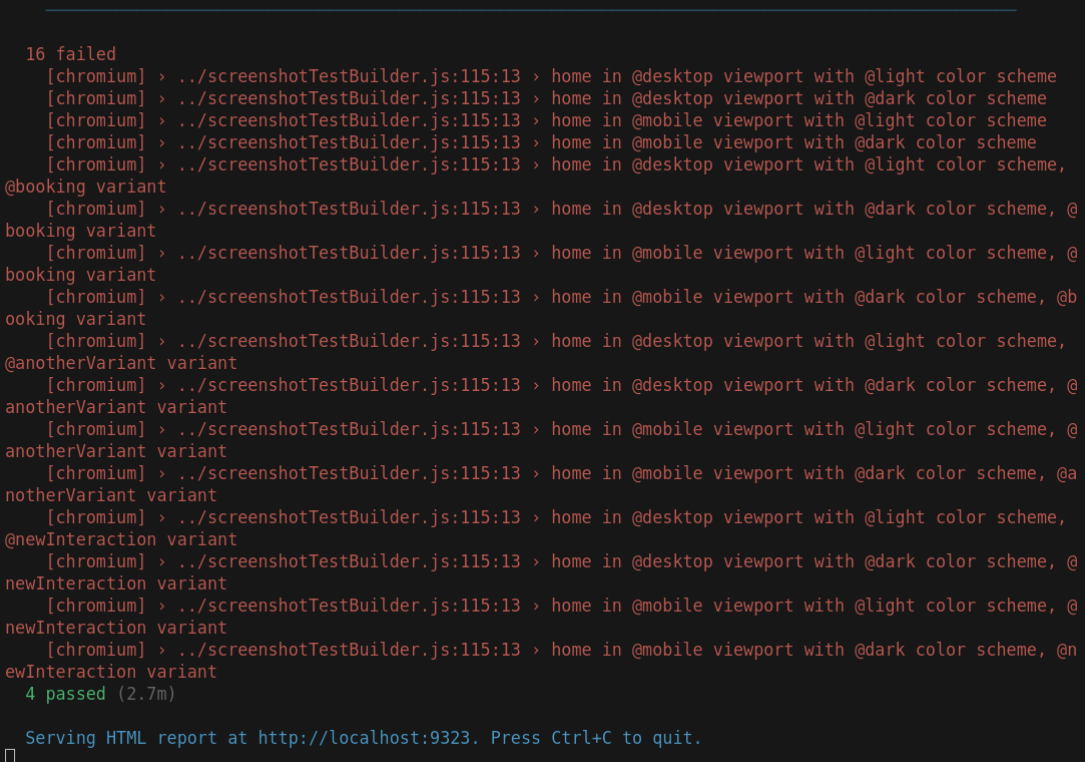
\includegraphics[width=0.80\textwidth]{e2e_console_test_log.png}
\caption{Fragment logu uruchomienia testów E2E w trybie konsolowym. Widoczne są m.in.\ błędy nieudanego testu zrzutu ekranu (16 testów niepowodzeń i 4 zakończone sukcesem).}
\label{fig:e2e-console-test-log}
\end{figure}

Na rysunku \ref{fig:e2e-console-test-log} widzimy przykładowy log z linii poleceń, gdzie \emph{Playwright} raportuje niezgodności względem oczekiwanego zrzutu ekranu (\texttt{toHaveScreenshot}). Przyczyny błędów mogą wynikać np.\ ze zmian w układzie strony lub dodania nowych elementów, co sprawia, że generowany obraz różni się od wzorca.

\subsection*{Raport nieudanego testu wizualnego}
Po zakończeniu testów w trybie \emph{UI} bądź w trybie \emph{console} (\emph{headless}), możliwe jest obejrzenie raportów w formacie HTML. Rysunek \ref{fig:e2e-report-web-test-log} ilustruje fragment takiego raportu, w którym \emph{Playwright} wskazuje różnice między oczekiwanym a aktualnym zrzutem ekranu.

\begin{figure}[H]
\centering
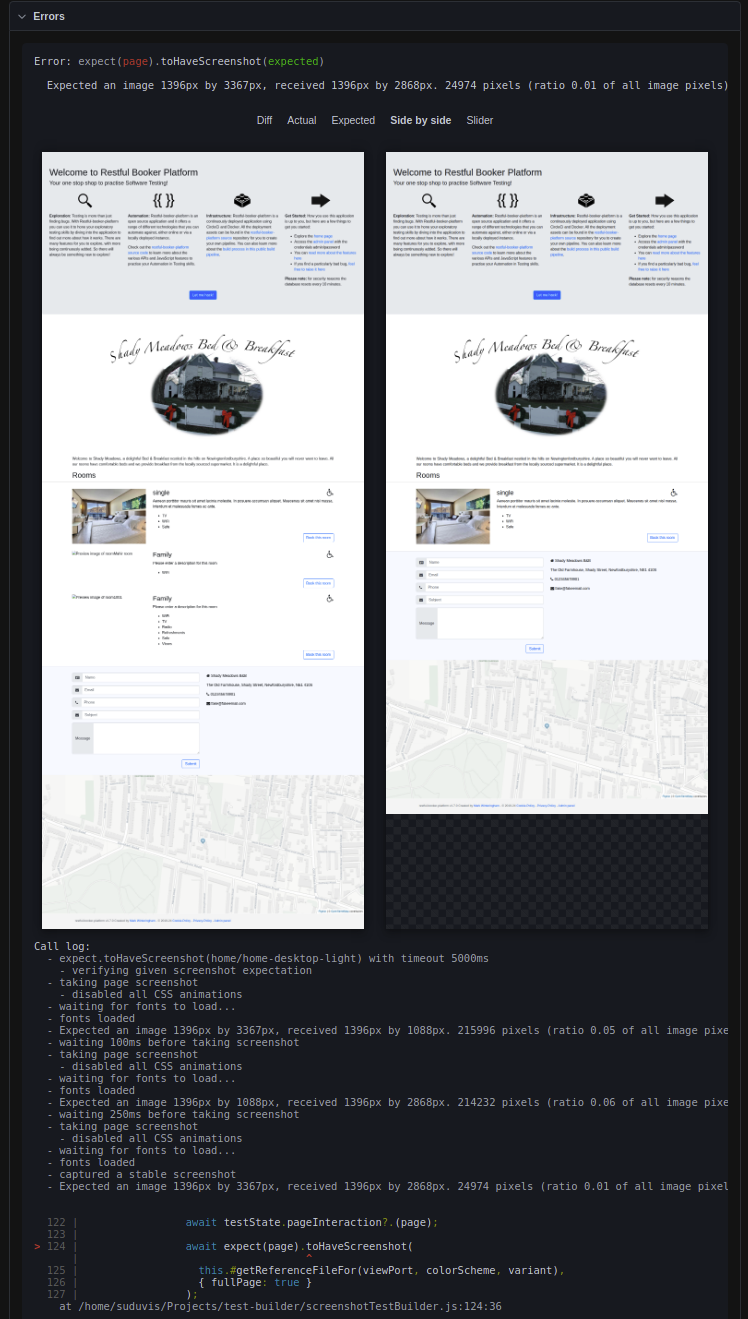
\includegraphics[width=0.90\textwidth]{e2e_report_web_test_log.png}
\caption{Raport \emph{Playwright} w przeglądarce – przykładowy błąd spowodowany różnicą w rozmiarach zrzutu ekranu.}
\label{fig:e2e-report-web-test-log}
\end{figure}

Z raportu (rys. \ref{fig:e2e-report-web-test-log}) wynika m.in.\ że oczekiwano obrazu o wymiarach \texttt{1396px x 3367px}, lecz w trakcie testu uzyskano \texttt{1396px x 2868px}. Tego typu różnica może wystąpić w sytuacji, gdy nie załadowała się dana sekcja strony albo zmieniono styl CSS powodujący inny rozmiar.

\subsection*{Przykładowy \emph{screenshot} testowanej aplikacji}

Poniżej zamieszczono przykładowy zrzut ekranu testowanej aplikacji (\texttt{home-desktop-light-booking-chromium.png}). Ten plik jest generowany w folderze \texttt{tests/home/} podczas uruchamiania testów \texttt{home.spec.js}. Zgodnie z konwencją nazewniczą:
\[
 \texttt{home-desktop-light-booking-chromium.png}
\]
oznacza, że jest to widok \texttt{home} w trybie \emph{desktop}, \emph{light} i wariancie \emph{booking}, uruchomionym w przeglądarce \emph{chromium}.

\begin{figure}[H]
\centering
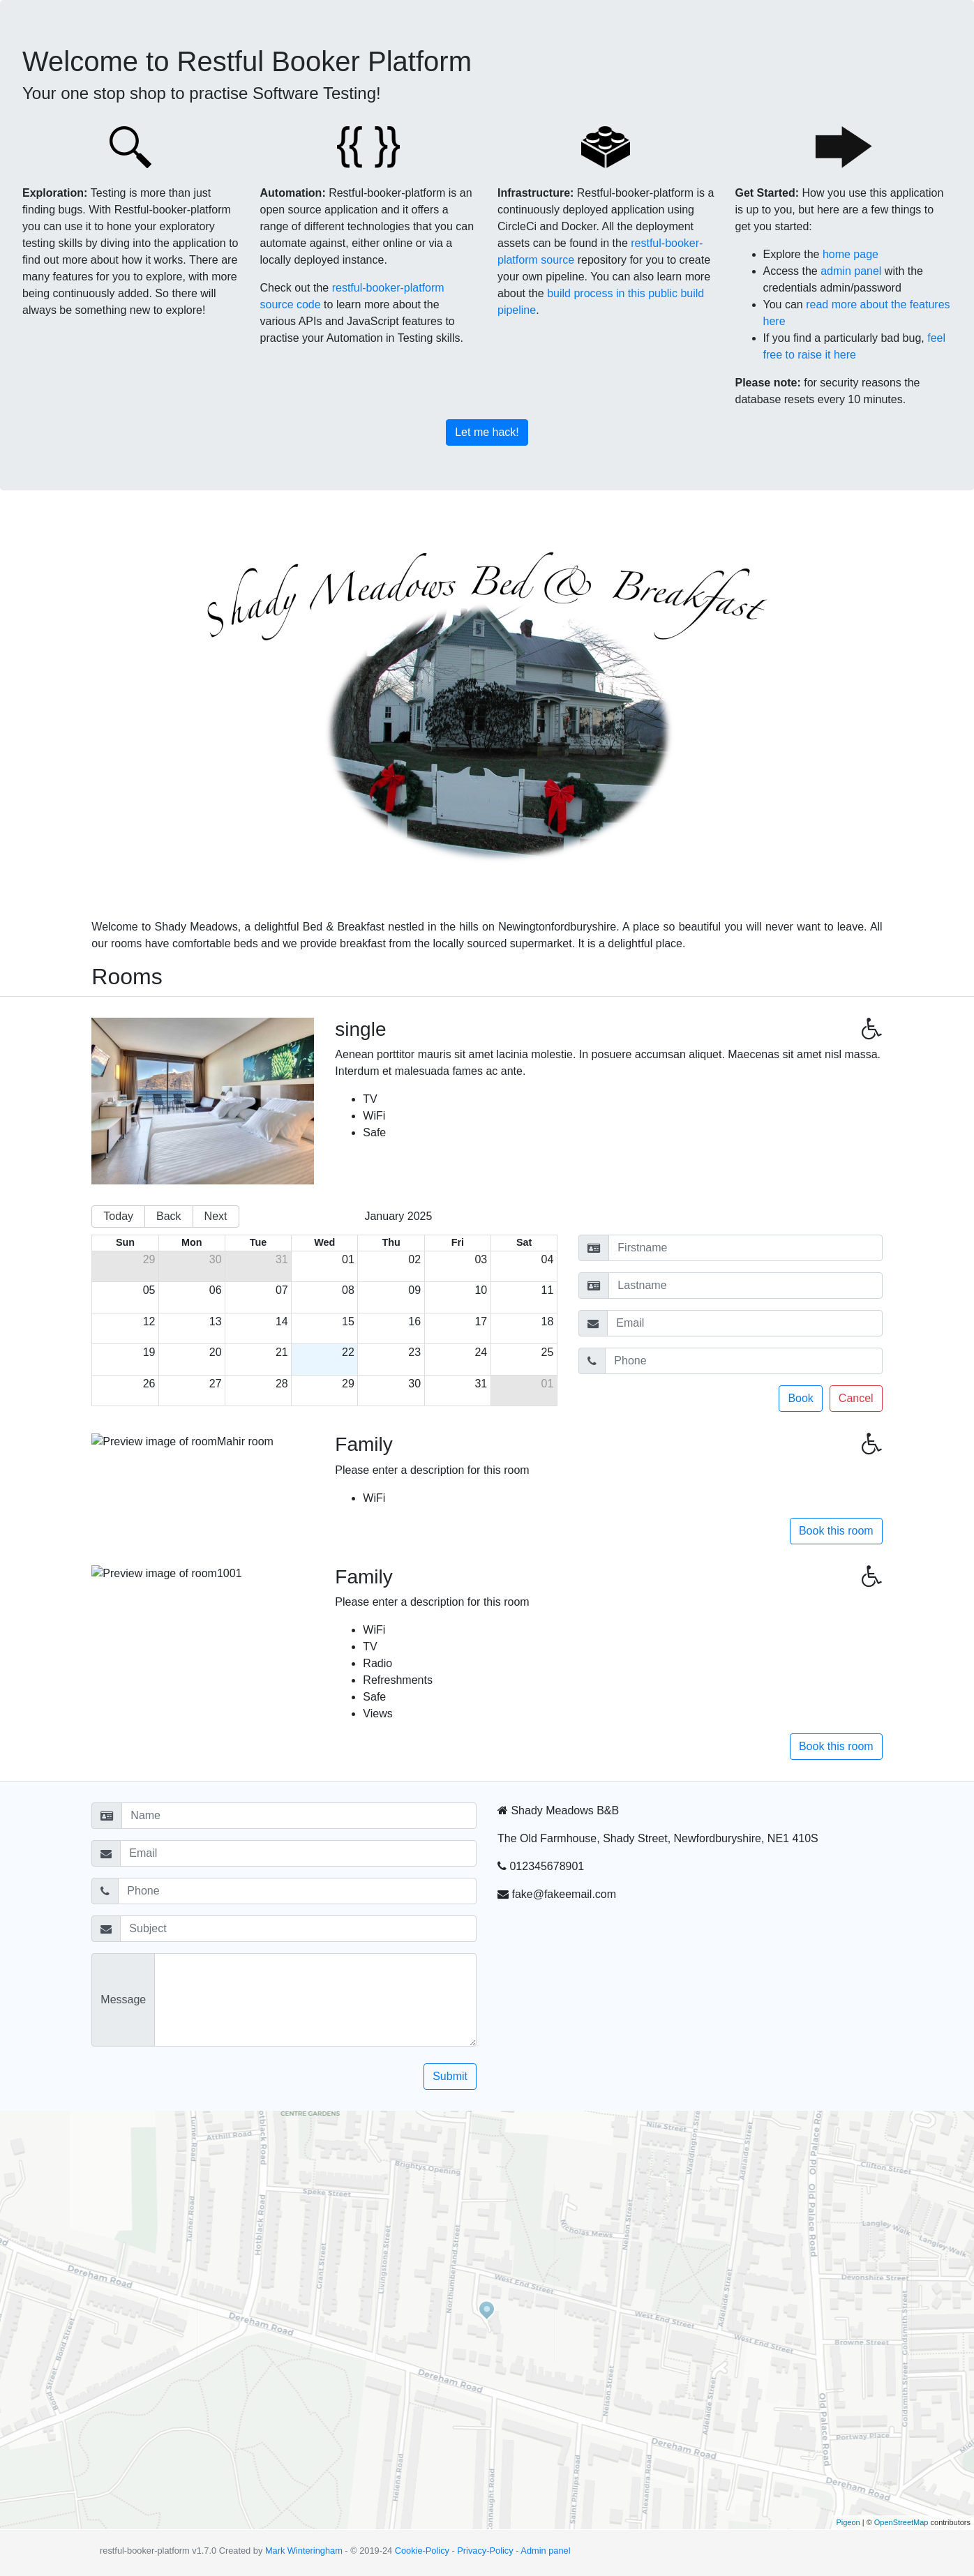
\includegraphics[width=0.36\textwidth]{home-desktop-light-booking-chromium.png}
\caption{Przykładowy screenshot aplikacji \texttt{home} (desktop, jasny motyw, wariant \emph{booking}).}
\label{fig:home-desktop-light-booking}
\end{figure}

\subsection*{Testy \texttt{mockApi} – przykłady sukcesu i błędu}

Poza samymi testami \emph{E2E} ważną częścią narzędzia jest weryfikacja plików \texttt{.mock.js} względem rzeczywistego API (komenda \texttt{npm run test:mock}). Rysunek \ref{fig:mock-test-sucess-log} przedstawia przykład poprawnych testów \texttt{mock}, a rysunek \ref{fig:mock-test-failure-log} pokazuje sytuację, gdy \texttt{mockApi} nie jest zgodne z aktualnym schematem serwera.

\begin{figure}[H]
\centering
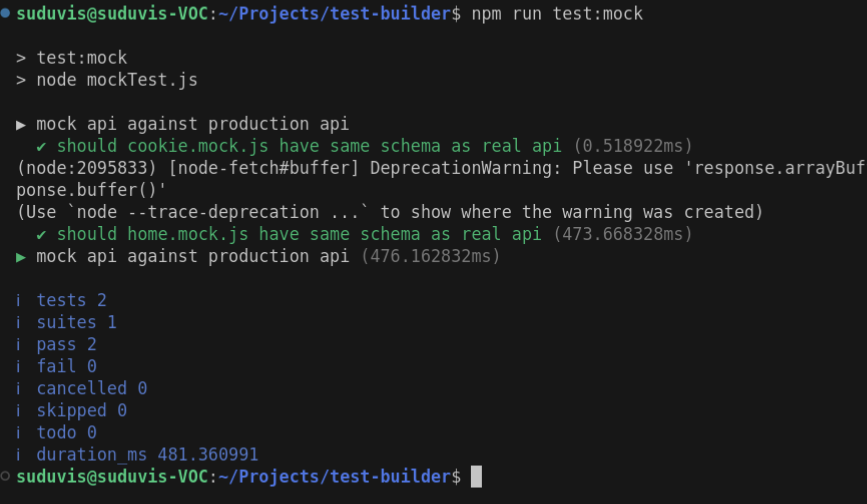
\includegraphics[width=0.80\textwidth]{mock_test_succes_log.png}
\caption{Przykład udanego uruchomienia testów \texttt{mockTest.js}, w którym zweryfikowano poprawność 2 plików \texttt{.mock.js}.}
\label{fig:mock-test-sucess-log}
\end{figure}

\begin{figure}[H]
\centering
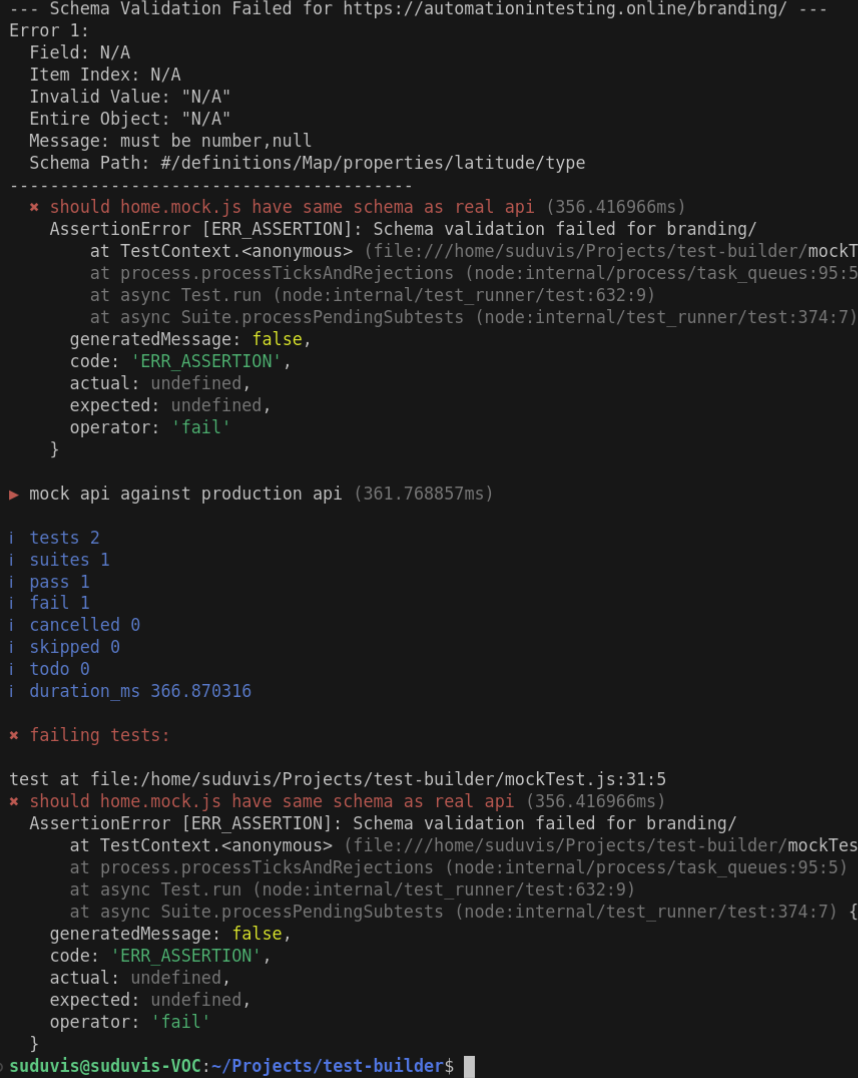
\includegraphics[width=0.80\textwidth]{mock_failure_test_log.png}
\caption{Przykład błędu w \texttt{mockTest.js} – struktura zwracanego \texttt{branding/} nie zgadza się z oczekiwaną (pole \texttt{latitude} nie jest typu \texttt{number/null}).}
\label{fig:mock-test-failure-log}
\end{figure}

Jak widać, dzięki \emph{mockTest} można w porę wykryć nieaktualne \texttt{mocki}, które mogłyby wprowadzać w błąd testy \emph{E2E}.

\subsection{Przykładowy kod \texttt{home.spec.js}}
\label{sec:home-spec-code}

Poniżej zamieszczono przykładowy plik testowy \texttt{home.spec.js}, w którym zdefiniowano trzy warianty testu (\emph{main}, \emph{booking}, \emph{newInteraction}). W każdym z nich można ustawić nieco inne interakcje (\texttt{setPageInteraction}) wykonywane przed zrobieniem zrzutu ekranu.

\begin{verbatim}
====== tests/home/home.spec.js ======
//@ts-check
import ScreenshotTest from '../../screenshotTestBuilder.js';

new ScreenshotTest()
  .forPage('/', 'home')
  .only()
  .test()
  .setPageInteraction(async (page) => {
    await page.getByRole('button', { name: 'Book this room' }).click();
  })
  .test('booking')
  .test('anotherVariant')
  .setPageInteraction(async (page) => {
    await page.getByTestId('ContactName').fill('hihihi');
  })
  .test('newInteraction');
\end{verbatim}

\noindent
Każdorazowe wywołanie metody \texttt{test('nazwa')} generuje serię testów wizualnych w różnych kombinacjach rozdzielczości i wariantów (definiowanych w \texttt{screenshotTestBuilder}). W efekcie otrzymujemy m.in.\ zrzuty ekranu w \emph{desktop/mobile}, trybie \emph{light/dark} oraz – opcjonalnie – w różnych przeglądarkach (\emph{chromium}, \emph{firefox}, \emph{webkit}).

\subsection{Przykładowy kod \texttt{home.mock.js}}
\label{sec:home-mock-code}

Poniżej pokazano część pliku \texttt{home.mock.js}, odpowiedzialnego za symulowanie odpowiedzi punktu \texttt{/branding/} oraz \texttt{/room/}. Zawiera on również definicję dwóch plików graficznych (bufor obrazu \texttt{room2.jpg} oraz \texttt{rbp-logo.jpg}), wczytywanych za pomocą \texttt{fs.readFileSync}.

\begin{verbatim}
====== mock-api/home/home.mock.js ======
import fs from 'fs';

const roomImage = fs.readFileSync(new URL('./room2.jpg', import.meta.url));
const rbpLogo = fs.readFileSync(new URL('./rbp-logo.jpg', import.meta.url));

const mockApi = {
  branding: {
    default: {
      endpoint: 'branding/',
      query: '',
      data: {
        name: 'Shady Meadows B&B',
        map: {
          latitude: 52.6351204,
          longitude: 1.2733774,
        },
        logoUrl: '/images/rbp-logo.jpg',
        description:
          'Welcome to Shady Meadows, a delightful Bed & Breakfast nestled ...',
        contact: {
          name: 'Shady Meadows B&B',
          address: 'The Old Farmhouse, Shady Street, Newfordburyshire, NE1 410S',
          phone: '012345678901',
          email: 'fake@fakeemail.com',
        },
      },
    },
  },
  room: {
    default: {
      endpoint: 'room/',
      query: '',
      data: {
        rooms: [
          {
            roomid: 1,
            roomName: '101',
            type: 'single',
            accessible: true,
            image: '/images/room2.jpg',
            description:
              'Aenean porttitor mauris sit amet lacinia molestie...',
            features: ['TV', 'WiFi', 'Safe'],
            roomPrice: 100,
          },
        ],
      },
    },
  },
  images: {
    room: {
      endpoint: 'images/room2.jpg',
      query: '',
      contentType: 'image/jpeg',
      data: roomImage,
    },
    logo: {
      endpoint: 'images/rbp-logo.jpg',
      query: '',
      contentType: 'image/jpeg',
      data: rbpLogo,
    },
  },
};

const mockApiPresets = {
  default: [
    mockApi['branding'].default,
    mockApi['room'].default,
    mockApi['images'].room,
  ],
};

export { mockApi, mockApiPresets };
\end{verbatim}

\noindent
Widzimy, że plik \texttt{home.mock.js} eksportuje \texttt{mockApiPresets.default}, dzięki czemu w \texttt{screenshotTestBuilder} można jednocześnie podmienić kilka endpointów (\texttt{/branding/}, \texttt{/room/}, \texttt{/images/room2.jpg}) w trakcie testu E2E, bez potrzeby odwoływania się do prawdziwej bazy danych czy usług backendowych.

\section{Integracja z procesem CI/CD}
\label{subsec:7.2}

W niniejszym podrozdziale przedstawiono przykładową konfigurację \texttt{.gitlab-ci.yml} w celu uruchamiania testów \texttt{e2e} oraz \texttt{mockTest} (zdefiniowanych w pliku \texttt{package.json}) w ramach pipeline w GitLab. Dzięki takiemu podejściu, przy każdym wprowadzeniu zmian w repozytorium, testy będą wykonywane automatycznie, co zapewni stałą kontrolę nad jakością aplikacji.

\begin{verbatim}
stages:
  - test

# Uruchamianie testów e2e za pomocą Playwright
test_e2e:
  stage: test
  image: mcr.microsoft.com/playwright:v1.49.1-jammy
  script:
    - npm ci
    - npm run test:e2e
  artifacts:
    when: always
    paths:
      - playwright-report
    expire_in: 1 day

# Uruchamianie mockTest w celu weryfikacji plików .mock.js
test_mock:
  stage: test
  image: node:18
  script:
    - npm ci
    - npm run test:mock
\end{verbatim}

\noindent
W powyższym przykładzie zdefiniowano jeden \emph{stage} o nazwie \texttt{test}, w ramach którego działają dwa zadania (\emph{jobs}):
\begin{itemize}
  \item \texttt{test\_e2e} -- pobiera zależności (\texttt{npm ci}), a następnie uruchamia testy end-to-end (\texttt{npm run test:e2e}) z wykorzystaniem obrazu Dockera, który zawiera środowisko \emph{Playwright}. Po zakończeniu testów artefakty (raporty i zrzuty ekranu) zostają zarchiwizowane (przechowywane przez 1 dzień) w zakładce \emph{Jobs} w GitLab.
  \item \texttt{test\_mock} -- także pobiera zależności, a następnie wywołuje \texttt{npm run test:mock}, które sprawdza poprawność plików \texttt{.mock.js} względem realnego API (m.in. przy pomocy \texttt{mockTest.js}). Jeśli w \texttt{mockApi} występują niezgodności, zadanie zakończy się niepowodzeniem.
\end{itemize}

\noindent
\textbf{Efekt działania pipeline:}  
Po zaktualizowaniu kodu w repozytorium GitLab automatycznie uruchamia oba zadania w kolejności zdefiniowanej w pliku \texttt{.gitlab-ci.yml}. W przypadku wykrycia błędów (zarówno w testach E2E, jak i w \texttt{mockTest}), pipeline zostaje oznaczony jako \emph{failed}, a deweloperzy mogą przejrzeć logi w GitLab, aby dowiedzieć się, które testy nie przeszły pomyślnie. W efekcie zapewniona jest ciągła walidacja jakości aplikacji: testy \emph{end-to-end} weryfikują rzeczywiste scenariusze działania w przeglądarce, zaś \emph{mockTest} gwarantuje zgodność plików \texttt{.mock.js} ze strukturą aktualnego API.

\chapter{Podsumowanie}
W niniejszej pracy przedstawiono koncepcję i implementację narzędzia wspomagającego tworzenie testów automatycznych dla aplikacji webowych. Podczas realizacji celu skupiono się na kilku aspektach: generowaniu testów z użyciem podejścia \emph{record-and-play} (\textit{Playwright codegen}), elastycznej konfiguracji \emph{mocków} API oraz integracji z pipeline’ami CI/CD. Projekt ma formę modułowego rozwiązania, w którym podstawową rolę odgrywa \texttt{screenshotTestBuilder} (klasa budująca testy wizualne) oraz \texttt{testManager} (narzędzie CLI do zarządzania plikami \texttt{.spec.js} i interakcjami testowymi).

\section{Wnioski końcowe}
Opracowane narzędzie pozwala tworzyć i utrzymywać testy w bardziej zorganizowany sposób, nawet w małych i średnich zespołach. Dzięki funkcji automatycznego nagrywania czynności (\emph{Playwright codegen}) programista nie musi ręcznie pisać skryptów testowych — zamiast tego może „nagrać” interakcje w przeglądarce i w prosty sposób wstawić je do \texttt{.spec.js} za pomocą \texttt{testManager}. Wprowadzenie \texttt{mockTest} z kolei ułatwia dbanie o aktualność \texttt{mocków} względem faktycznego API, co zmniejsza ryzyko, że testy staną się nieadekwatne do stanu produkcyjnego.  

Największym wyzwaniem okazało się zapewnienie spójności między wieloma komponentami (m.in. \texttt{screenshotTestBuilder}, \texttt{mockApi}, \texttt{testManager}, \texttt{codegen}) oraz umożliwienie ich rozszerzania w przyszłości. Istotnym wnioskiem jest też fakt, że jakość i stabilność testów wciąż w dużej mierze zależą od świadomego projektowania scenariuszy i ich regularnej aktualizacji — narzędzie automatyzuje wiele zadań, lecz nie zastępuje w pełni testera czy programisty.

\section{Możliwości dalszego rozwoju}
\begin{itemize}
    \item \textbf{Integracja z innymi frameworkami}: Choć obecnie wykorzystano \emph{Playwright}, narzędzie można wzbogacić o mechanizmy wspierające inne biblioteki (np. \emph{Cypress}), zapewniając szerszy wybór w zależności od preferencji zespołu.
    \item \textbf{Rozszerzona edycja interakcji}: \texttt{testManager} mógłby oferować interfejs wizualny (np. w trybie webowym) do modyfikacji sekwencji kroków, z podglądem wszystkich akcji i możliwością ich przestawiania.
    \item \textbf{Dodatkowe formy testów wizualnych}: Obecnie generowane są zrzuty ekranu pełnej strony. Cennym usprawnieniem może być porównywanie wybranych elementów interfejsu (np. wycinek z modalem) lub tworzenie animowanych \emph{gifów} pokazujących interakcje krok po kroku.
    \item \textbf{Analiza regresji wizualnej w chmurze}: Można zintegrować narzędzie z zewnętrznymi usługami do porównywania obrazów w chmurze (np. \emph{Applitools}), aby odciążyć infrastrukturę lokalną i usprawnić raportowanie różnic.
    \item \textbf{Weryfikacja dostępności (Accessibility)}: Istnieje potencjał do rozszerzenia testów o automatyczną analizę dostępności (np. integracja z \texttt{@axe-core/playwright}), co umożliwi wychwytywanie problemów już na etapie codziennego \emph{builda}.
    \item \textbf{Zaawansowane generowanie testów}: Oprócz prostego \emph{record-and-play} można wprowadzić tryb \emph{Model-Based Testing}, w którym narzędzie generowałoby wiele ścieżek przejścia w aplikacji w sposób systematyczny i pokrywający większą liczbę stanów.
\end{itemize}

Proponowane kierunki rozwoju pozwoliłyby jeszcze bardziej rozszerzyć możliwości narzędzia i uczynić je atrakcyjniejszym zarówno dla zespołów wdrażających podstawową automatyzację testów, jak i tych, które stawiają na kompleksowe, wielopoziomowe podejście do zapewniania jakości.

\begin{thebibliography}{9}
    \bibitem{roman2024} Roman, A., \& Zmitrow, K. (2024). \textit{Testowanie oprogramowania w praktyce: studium przypadków 2.0}.
    \bibitem{osherove2024} Osherove, R. (2024). \textit{Testy jednostkowe: świat niezawodnych aplikacji}.
    \bibitem{roman2024_case} Roman, A., \& Zmitrow, K. (2024). \textit{Testowanie oprogramowania w praktyce: studium przypadków}.
    \bibitem{roman2024_quality} Roman, A. (2024). \textit{Testowanie i jakość oprogramowania: modele, techniki, narzędzia}.
    \bibitem{circleci} CircleCI. (n.d.). What is End-to-End Testing? Pozyskano z \url{https://circleci.com/blog/what-is-end-to-end-testing/}
    \bibitem{playwright} Microsoft Playwright. (n.d.). Introduction to Playwright. Pozyskano z \url{https://playwright.dev/docs/intro}
\end{thebibliography}

\end{document}